%-------------------------------------------------------------------------------
% This file provides a skeleton ATLAS note.
% \pdfinclusioncopyfonts=1
% This command may be needed in order to get \ell in PDF plots to appear. Found in
% https://tex.stackexchange.com/questions/322010/pdflatex-glyph-undefined-symbols-disappear-from-included-pdf
%-------------------------------------------------------------------------------
% Specify where ATLAS LaTeX style files can be found.
\newcommand*{\ATLASLATEXPATH}{latex/}
% Use this variant if the files are in a central location, e.g. $HOME/texmf.
% \newcommand*{\ATLASLATEXPATH}{}
%-------------------------------------------------------------------------------
%\documentclass[USenglish,texlive=2016,cernpreprint,NOTE,paper=A4]{\ATLASLATEXPATH atlasdoc}
\documentclass[NOTE, atlasdraft=true, texlive=2016, UKenglish]{\ATLASLATEXPATH atlasdoc}
%\usepackage{\ATLASLATEXPATH atlasphysics}
\usepackage{float}
\usepackage{numprint}
%\usepackage{siunitx}
\usepackage{changepage}
\usepackage{euler}\usepackage{pgf}
%\usepackage[backend=biber]{biblatex}
%\usepackage{natbib}
\usepackage{geometry}
\usepackage{pdflscape}
\usepackage{longtable}
\DeclareOldFontCommand{\bf}{\normalfont\bfseries}{\mathbf}
% The language of the document must be set: usually UKenglish or USenglish.
% british and american also work!
% Commonly used options:
%  atlasdraft=true|false This document is an ATLAS draft.
%  texlive=YYYY          Specify TeX Live version (2016 is default).
%  coverpage             Create ATLAS draft cover page for collaboration circulation.
%                        See atlas-draft-cover.tex for a list of variables that should be defined.
%  cernpreprint          Create front page for a CERN preprint.
%                        See atlas-preprint-cover.tex for a list of variables that should be defined.
%  NOTE                  The document is an ATLAS note (draft).
%  PAPER                 The document is an ATLAS paper (draft).
%  CONF                  The document is a CONF note (draft).
%  PUB                   The document is a PUB note (draft).
%  BOOK                  The document is of book form, like an LOI or TDR (draft)
%  txfonts=true|false    Use txfonts rather than the default newtx
%  paper=a4|letter       Set paper size to A4 (default) or letter.

%-------------------------------------------------------------------------------
% Extra packages:
%\usepackage{\ATLASLATEXPATH atlaspackage}
\usepackage[subfigure]{\ATLASLATEXPATH atlaspackage}
%\usepackage[biblatex=false]{\ATLASLATEXPATH atlaspackage}
% Commonly used options:
%  biblatex=true|false   Use biblatex (default) or bibtex for the bibliography.
%  backend=bibtex        Use the bibtex backend rather than biber.
%  subfigure|subfig|subcaption  to use one of these packages for figures in figures.
%  minimal               Minimal set of packages.
%  default               Standard set of packages.
%  full                  Full set of packages.
%-------------------------------------------------------------------------------
% Style file with biblatex options for ATLAS documents.
%\usepackage[biblatex=true]{\ATLASLATEXPATH atlasbiblatex}

% Package for creating list of authors and contributors to the analysis.
\usepackage{\ATLASLATEXPATH atlascontribute}

% Useful macros
\usepackage{\ATLASLATEXPATH atlasphysics}
% See doc/atlas_physics.pdf for a list of the defined symbols.
% Default options are:
%   true:  journal, misc, particle, unit, xref
%   false: BSM, heppparticle, hepprocess, hion, jetetmiss, math, process, other, texmf
% See the package for details on the options.

% Files with references for use with biblatex.
% Note that biber gives an error if it finds empty bib files.
\addbibresource{bib/wz_heavy_flavor.bib}
\addbibresource{bib/ATLAS.bib}
\addbibresource{bib/CMS.bib}
\addbibresource{bib/ConfNotes.bib}
\addbibresource{bib/PubNotes.bib}

% Paths for figures - do not forget the / at the end of the directory name.
\graphicspath{{logos/}{figures/}}

% Add you own definitions here (file wz_heavy_flavor-defs.sty).
\usepackage{wz_heavy_flavor-defs}

%-------------------------------------------------------------------------------
% Generic document information
%-------------------------------------------------------------------------------

% Title, abstract and document 
%-------------------------------------------------------------------------------
% This file contains the title, author and abstract.
% It also contains all relevant document numbers used for an ATLAS note.
%-------------------------------------------------------------------------------

% Title
\AtlasTitle{WZ + Heavy Flavor Production in pp collisions at $\sqrt{s}$ = 13 TeV}

% Draft version:
% Should be 1.0 for the first circulation, and 2.0 for the second circulation.
% If given, adds draft version on front page, a 'DRAFT' box on top of each other page, 
% and line numbers.
% Comment or remove in final version.
\AtlasVersion{0.1}

% Abstract - % directly after { is important for correct indentation
\AtlasAbstract{%
        A measurement of the cross-section for production of WZ with an associated heavy flavor jet is performed using 140 $fb^{-1}$ of proton-proton collision data at $\sqrt{s} =$ 13 TeV from the ATLAS experiment at the LHC. A measurement of the fully leptonic decay mode, $WZ\rightarrow l\nu ll$, is performed. The cross-section of WZ + $b$ and WZ + charm in various fiducial regions is measured.
}

% Author - this does not work with revtex (add it after \begin{document})
\author{The ATLAS Collaboration}

% Authors and list of contributors to the analysis
% \AtlasAuthorContributor also adds the name to the author list
% Include package latex/atlascontribute to use this
% Use authblk package if there are multiple authors, which is included by latex/atlascontribute
% \usepackage{authblk}
% Use the following 3 lines to have all institutes on one line
% \makeatletter
% \renewcommand\AB@affilsepx{, \protect\Affilfont}
% \makeatother
% \renewcommand\Authands{, } % avoid ``. and'' for last author
% \renewcommand\Affilfont{\itshape\small} % affiliation formatting
% \AtlasAuthorContributor{First AtlasAuthorContributor}{a}{Author's contribution.}
% \AtlasAuthorContributor{Second AtlasAuthorContributor}{b}{Author's contribution.}
% \AtlasAuthorContributor{Third AtlasAuthorContributor}{a}{Author's contribution.}
% \AtlasContributor{Fourth AtlasContributor}{Contribution to the analysis.}
% \author[a]{First Author}
% \author[a]{Second Author}
% \author[b]{Third Author}
% \affil[a]{One Institution}
% \affil[b]{Another Institution}

% If a special author list should be indicated via a link use the following code:
% Include the two lines below if you do not use atlasstyle:
% \usepackage[marginal,hang]{footmisc}
% \setlength{\footnotemargin}{0.5em}
% Use the following lines in all cases:
% \usepackage{authblk}
% \author{The ATLAS Collaboration%
% \thanks{The full author list can be found at:\newline
%   \url{https://atlas.web.cern.ch/Atlas/PUBNOTES/ATL-PHYS-PUB-2017-007/authorlist.pdf}}
% }

% ATLAS reference code, to help ATLAS members to locate the paper
%\AtlasAuthorContributor{Aaron Webb}{a}{Main analyser. Responsible for ntuple production, fits, and note writing.}
%\AtlasAuthorContributor{Peter Onyisi}{a}{Advisor to Aaron Webb. Analysis design and implementation strategy.} 
%\AtlasAuthorContributor{Heather Russell}{b}{EWK group convener. Note editing, developing analysis strategy.}
%\AtlasAuthorContributor{Philip Sommer}{c}{EWK group convener. Note editing, developing analysis strategy.}

%\affil[a]{Univ. of Texas at Austin}
%\affil[b]{McGill University}
%\affil[c]{Univ. of Sheffield}

\AtlasRefCode{ATL-COM-PHYS-2019-962}

% ATLAS note number. Can be an COM, INT, PUB or CONF note
% \AtlasNote{ATLAS-CONF-2017-XXX}
% \AtlasNote{ATL-PHYS-PUB-2017-XXX}
% \AtlasNote{ATL-COM-PHYS-2017-XXX}

% Author and title for the PDF file
\hypersetup{pdftitle={ATLAS document},pdfauthor={The ATLAS Collaboration}}

%-------------------------------------------------------------------------------
% Content
%-------------------------------------------------------------------------------
\begin{document}

\maketitle

\tableofcontents

% List of contributors - print here or after the Bibliography.
\PrintAtlasContribute{0.30}
\clearpage

%-------------------------------------------------------------------------------                                     
\section{Introduction}
\label{sec:intro}

The production of $WZ$ in association with a heavy flavor jet represents an important background for many major analyses. This includes any process with multiple leptons and b-jets in the final state, such as $t\bar{t}H$, $t\bar{t}W$, and $t\bar{t}Z$. While precise measurements have been made of inclusive $WZ$ production \cite{WZ_36}, $WZ$ + heavy flavor remains poorly understood. This is largely because the QCD processes involved in the production of the b-jet make it difficult to simulate accurately. This introduces a large uncertainty for analyses that include this process as a background.  

We perform a study of the fully leptonic decay mode of this channel; that is, events where both the W and Z decay leptonically. Because WZ has no associated jets at leading order, while the major backgrounds for this channel tend to have high jet multiplicity, events with more than two jets are rejected. This gives a final state signature of three leptons and one or two jets.

Events that meet a preselection criteria are sorted into regions based on the b-taggin score of their associated jets. This is done to separate $WZ$ + b-jet events from $WZ$ + charm and $WZ$ + light jets. These regions are fit to data in order make a more accurate estimate of the contribution of $WZ$ + heavy-flavor, where heavy-flavor jets include b-jets and charm jets. The full Run-2 dataset collected by the ATLAS detector, representing 139 $fb^{-1}$ of data from pp collisions at $\sqrt{s} = 13$ TeV, is used for this study.

The fiducial volume at particle level is defined based on the number of stable leptons and jets in each event. Three light leptons with total charge $\pm$1 and one or two associated jets are required. Only leptons which do not originate from hadron or $\tau$ decays are considered. The phase space definitions use dressed kinematics of the final state particles. Leptons are dressed by summing the momentum of photons within a cone of $\Delta R < 0.1$ of the lepton to correct the leptons energy. Particle level jets are reconstructed using the anti-$k_t$ algorithm with a radius of $R=0.4$. The kinematic selection applied to these objects is summarized below:

\begin{itemize}
\item Three light leptons with total charge $\pm$1, $|\eta| < 2.5$
\item OS lepton with \pt$>$10 GeV, SS leptons with \pt$>$20 GeV
\item One OSSF lepton pair with $|M(ll)-91.2\ GeV| < 10\ GeV$
\item One or two associated truth jets with $p_T >$25 GeV, $|\eta| < 2.5$, $R<0.4$
%\item At least one truth b-jet or one charm jet
\end{itemize}

The result of the fit is used to extract the cross-section in this fiducial region for WZ + $b$ and WZ + $c$ with one associated jet, and WZ + $b$ and WZ + $c$ with two associated jets, where the number and flavor of the jets is determined at particle level. Events with both charm and b-jets are counted as WZ + $b$. The analysis reports a cross-section measurement of WZ + $b$ and WZ + $c$, along with their correlations, for both 1-jet and 2-jet exclusive regions. Normalization factors, representing how the MC prediction differs from the observed result, are also reported.

Section \ref{sec:data} details the data and Monte Carlo (MC) samples used in the analysis. The reconstruction of various physics objects is described in Section \ref{sec:obj}. Section \ref{sec:evt_selection} describes the event selection applied to these samples, along the definitions of the various regions used in the fit. The multivariate analysis techniques used to separate the tZ background from WZ + heavy flavor are described in Section \ref{sec:tZ_bdt}. Section \ref{sec:sys} describes the various sources of systematic uncertainties considered in the fit. Finally, the results of the analysis are summarized in Section \ref{sec:results}, followed by a brief conclusion in Section \ref{sec:conclusion}.



%-------------------------------------------------------------------------------

%-------------------------------------------------------------------------------                                             
\section{The ATLAS Detector}
\label{sec:ATLAs}
The ATLAS detector \cite{} at the LHC is a general purpose detector that covers nearly the entire solid angle around the collision point. It consists of several concentric subdectors: The inner tracking detector, electromagnetic and hadronic calorimeters, and a muon spectrometer. The inner detector is made up of a high-granularity silicon pixel detector, designed to reconstruct the tracks of charged particles in a range of $|\eta|< 2.5$, and a transition radiation tracker which provides additional tracking and electron identification information for $|\eta|< 2.0$ \cite{}. A 2 T axial magnetic field is produced in the inner detector, in order to bend the path of charged particles. The calorimeter system cover a pseudorapidity range of $|\eta|< 4.9$, with a a lead/liquid-argon (LAr) electromagnetic calorimeter covering $|\eta|< 3.2$, and a steel/scintillator-tile hadronic calorimeter. The rest of the solid-angle coverage of the calorimeter system comes from forward copper/LAr and tungsten/LAr modules. The muon spectrometer measures muons with $|\eta|< 2.7$ using several layered tracking chambers placed within a magnetic field of approximately 0.5 T. A two-level trigger system \cite{} is used to reduce the event rate from 40 MHz to around 1 kHz, using a hardware based Level-1 trigger, followed by a second software based High-Level Trigger (HLT).

%-------------------------------------------------------------------------------  

%-------------------------------------------------------------------------------
%\section{Introduction}
%\label{sec:intro}
%
The production of $WZ$ in association with a heavy flavor jet represents an important background for many major analyses. This includes any process with multiple leptons and b-jets in the final state, such as $t\bar{t}H$, $t\bar{t}W$, and $t\bar{t}Z$. While precise measurements have been made of inclusive $WZ$ production \cite{WZ_36}, $WZ$ + heavy flavor remains poorly understood. This is largely because the QCD processes involved in the production of the b-jet make it difficult to simulate accurately. This introduces a large uncertainty for analyses that include this process as a background.  

We perform a study of the fully leptonic decay mode of this channel; that is, events where both the W and Z decay leptonically. Because WZ has no associated jets at leading order, while the major backgrounds for this channel tend to have high jet multiplicity, events with more than two jets are rejected. This gives a final state signature of three leptons and one or two jets.

Events that meet a preselection criteria are sorted into regions based on the b-taggin score of their associated jets. This is done to separate $WZ$ + b-jet events from $WZ$ + charm and $WZ$ + light jets. These regions are fit to data in order make a more accurate estimate of the contribution of $WZ$ + heavy-flavor, where heavy-flavor jets include b-jets and charm jets. The full Run-2 dataset collected by the ATLAS detector, representing 139 $fb^{-1}$ of data from pp collisions at $\sqrt{s} = 13$ TeV, is used for this study.

The fiducial volume at particle level is defined based on the number of stable leptons and jets in each event. Three light leptons with total charge $\pm$1 and one or two associated jets are required. Only leptons which do not originate from hadron or $\tau$ decays are considered. The phase space definitions use dressed kinematics of the final state particles. Leptons are dressed by summing the momentum of photons within a cone of $\Delta R < 0.1$ of the lepton to correct the leptons energy. Particle level jets are reconstructed using the anti-$k_t$ algorithm with a radius of $R=0.4$. The kinematic selection applied to these objects is summarized below:

\begin{itemize}
\item Three light leptons with total charge $\pm$1, $|\eta| < 2.5$
\item OS lepton with \pt$>$10 GeV, SS leptons with \pt$>$20 GeV
\item One OSSF lepton pair with $|M(ll)-91.2\ GeV| < 10\ GeV$
\item One or two associated truth jets with $p_T >$25 GeV, $|\eta| < 2.5$, $R<0.4$
%\item At least one truth b-jet or one charm jet
\end{itemize}

The result of the fit is used to extract the cross-section in this fiducial region for WZ + $b$ and WZ + $c$ with one associated jet, and WZ + $b$ and WZ + $c$ with two associated jets, where the number and flavor of the jets is determined at particle level. Events with both charm and b-jets are counted as WZ + $b$. The analysis reports a cross-section measurement of WZ + $b$ and WZ + $c$, along with their correlations, for both 1-jet and 2-jet exclusive regions. Normalization factors, representing how the MC prediction differs from the observed result, are also reported.

Section \ref{sec:data} details the data and Monte Carlo (MC) samples used in the analysis. The reconstruction of various physics objects is described in Section \ref{sec:obj}. Section \ref{sec:evt_selection} describes the event selection applied to these samples, along the definitions of the various regions used in the fit. The multivariate analysis techniques used to separate the tZ background from WZ + heavy flavor are described in Section \ref{sec:tZ_bdt}. Section \ref{sec:sys} describes the various sources of systematic uncertainties considered in the fit. Finally, the results of the analysis are summarized in Section \ref{sec:results}, followed by a brief conclusion in Section \ref{sec:conclusion}.



%-------------------------------------------------------------------------------

%-------------------------------------------------------------------------------
\section{Data and Monte Carlo Samples}
\label{sec:data}

%Both data and Monte Carlo samples used in this analysis were prepared in the \verb|xAOD| format, which was used to produce a \verb|DxAOD| sample in the \verb|HIGG8D1| derivation framework. The \verb|HIGG8D1| framework is designed for the $t\bar{t}H$ multi-lepton analysis, which targets events with multiple leptons as well as tau hadrons. This framework skims the dataset to remove unneeded variables as well as entire events. Events are removed from the derivations that do not meet the following selection:

%\begin{itemize}
%    \item at least two light leptons within a range $|\eta|$<2.6, with leading lepton $p_{T}$ > 15 GeV and subleading lepton $p_{T}$ > 5 GeV
%    \item at least one light lepton with $p_{T}$ > 15 GeV within a range $|\eta|$<2.6, and at least two hadronic taus with $p_{T}$ > 15 GeV.
%\end{itemize}

%Samples were then generated from these \verb|HIGG8D1| derivations with p-tag of p4134 for data and p4133 for Monte Carlo using AnalysisBase version 21.2.127 modified to include custom variables.

\subsection{Data Samples}

This study uses a sample of proton-proton collision data collected by the ATLAS detector from 2015 through 2018 at an energy of $\sqrt{s} = 13$ TeV, which represents an integrated luminosity of 139 $fb^{-1}$ \cite{lumi}. This data set was collected with a bunch-crossing rate of 25 ns. All data used in this analysis was verified by data quality checks \cite{PERF-2010-01}.

\subsection{Monte Carlo Samples}

Several different generators were used to produce Monte Carlo simulations of the signal and background processes. For all samples, the response of the ATLAS detector is simulated using \textsc{Geant4} \cite{GEANT4}. The WZ signal samples are simulated using Sherpa 2.2.2 \cite{sherpa}. Specific information about the Monte Carlo samples being used can be found in Table \ref{tbl:evgen}. 

\begin{table}[H]
\begin{center}
\caption{\label{tbl:evgen} The configurations used for event generation of signal and background processes, including the event generator, matrix element (ME) order, parton shower algorithm, and parton distribution function (PDF). }
 \resizebox{\textwidth}{!}{
\begin{tabular}{llllll}
\hline\hline
Process & Event generator & ME order & Parton Shower & PDF   \\
\hline
$WZ$, $ZZ$, $WW$ & \textsc{Sherpa} 2.2.2
& MEPS NLO & \textsc{Sherpa} & CT10 \cite{ct10} \\
$t Z$ & \textsc{MG5\_aMC} \cite{Alwall:2014hca} & NLO & \textsc{Pythia} 8  & CTEQ6L1  \\
$\ttbar W$ & \textsc{MG5\_aMC} & NLO & \textsc{Pythia} 8 & NNPDF 3.0 NLO \\
& (\textsc{Sherpa} 2.1.1) & (LO multileg) & (\textsc{Sherpa}) & (NNPDF 3.0 NLO)  \\
$\ttbar (Z/\gamma^* \to ll)$ & \textsc{MG5\_aMC} & NLO & \textsc{Pythia} 8 & NNPDF 3.0 NLO  \\
$t\bar{t}H$ & \textsc{MG5\_aMC} & NLO & \textsc{Pythia} 8\ & NNPDF 3.0 NLO \cite{Ball:2014uwa} \\
     & (\textsc{MG5\_aMC}) & (NLO) & (\textsc{Herwig++}) \cite{Bahr:2008pv} & (CT10 \cite{ct10})  \\
$tHqb$ & \textsc{MG5\_aMC} & LO & \textsc{Pythia} 8 & CT10  \\
$tHW$ & \textsc{MG5\_aMC} & NLO & \textsc{Herwig++}  & CT10  \\
& (\textsc{Sherpa} 2.1.1) & (LO multileg) & (\textsc{Sherpa}) & (NNPDF 3.0 NLO)  \\
$t W Z$ & \textsc{MG5\_aMC} & NLO & \textsc{Pythia} 8 & NNPDF 2.3 LO   \\
$t\bar t t$, $t\bar t t\bar t$ & \textsc{MG5\_aMC} & LO & \textsc{Pythia} 8 & NNPDF 2.3 LO \cite{Ball:2012cx} \\
$t\bar t W^+ W^-$ & \textsc{MG5\_aMC} & LO & \textsc{Pythia} 8 & NNPDF 2.3 LO\\
$\ttbar$ & \textsc{Powheg-BOX v2} \cite{powhegtt} & NLO & \textsc{Pythia} 8 & NNPDF 3.0 NLO  \\
$\ttbar\gamma$ & \textsc{MG5\_aMC} & LO & \textsc{Pythia} 8 & NNPDF 2.3 LO \\
$s$-, $t$-channel, & \textsc{Powheg-BOX v1} \cite{powhegstp}& NLO & \textsc{Pythia} 6 & CT10 \\
 $Wt$ single top & & & &  \\
$qqVV$, $VVV$ & &   \\
$Z \to l^+l^-$ & \textsc{Sherpa} 2.2.1 & MEPS NLO  & \textsc{Sherpa} & NNPDF 3.0 NLO \\
\hline\hline
\end{tabular}
}
\end{center}
\end{table}

%-------------------------------------------------------------------------------

%-------------------------------------------------------------------------------
\section{Object Reconstruction}
\label{sec:obj}

All regions defined in this analysis share a common lepton, jet, and overall event preselection. This preselection is detailed here; the selection used to define the various fit regions is described in section \ref{sec:signal_region}.

\subsection{Trigger}

Events are required to be selected by dilepton triggers, as summarized in table \ref{tbl:trigger}. 

\begin{table}[h!]
 \begin{center}
   \begin{tabular}{cc}
     \toprule
                  & Dilepton triggers (2015) \\
     \midrule
      $\mu\mu$ (asymm.)          & \verb!HLT_mu18_mu8noL1! \\
      $ee$ (symm.)               & \verb!HLT_2e12_lhloose_L12EM10VH! \\
      $e\mu,\mu e$ ($\sim$symm.) & \verb!HLT_e17_lhloose_mu14! \\
     \bottomrule
                       & Dilepton triggers (2016) \\
     \midrule
      $\mu\mu$ (asymm.)                   & \verb!HLT_mu22_mu8noL1! \\
      $ee$ (symm.)                        & \verb!HLT_2e17_lhvloose_nod0! \\
      $e\mu,\mu e$ ($\sim$symm.)          & \verb!HLT_e17_lhloose_nod0_mu14! \\
     \bottomrule

                  & Dilepton triggers (2017) \\
     \midrule
      $\mu\mu$ (asymm.)                   & \verb!HLT_mu22_mu8noL1! \\
      $ee$ (symm.)                        & \verb!HLT_2e24_lhvloose_nod0! \\
      $e\mu,\mu e$ ($\sim$symm.)          & \verb!HLT_e17_lhloose_nod0_mu14! \\
     \bottomrule
                  & Dilepton triggers (2018) \\
     \midrule
      $\mu\mu$ (asymm.)                   & \verb!HLT_mu22_mu8noL1! \\
      $ee$ (symm.)                        & \verb!HLT_2e24_lhvloose_nod0! \\
      $e\mu,\mu e$ ($\sim$symm.)          & \verb!HLT_e17_lhloose_nod0_mu14! \\ 
      \bottomrule
   \end{tabular}
   \caption{\label{tbl:trigger} List of lowest $p_{T}$-threshold, un-prescaled dilepton triggers used for 2015-2018 data taking.}
 \end{center}
\end{table}

\subsection{Light leptons}
\label{subsec:leps}

Electron candidates are reconstructed from energy clusters in the electromagnetic calorimeter that are associated with charged particle tracks reconstructed in the inner detector~\cite{ATLAS-CONF-2016-024}.  Electron candidates are required to have $\pt > 10$ GeV and $|\eta_\textrm{cluster}| < 2.47$. Candidates in the transition region between different electromagnetic calorimeter components, $1.37 < |\eta_\textrm{cluster}| < 1.52$, are rejected. A multivariate likelihood discriminant combining shower shape and track information is used to distinguish real electrons from hadronic showers (fake electrons). To further reduce the non-prompt electron contribution, the track is required to be consistent with originating from the primary vertex; requirements are imposed on the transverse impact parameter significance ($|d_0|/\sigma_{d_0}$) and the longitudinal impact parameter ($|\Delta z_0 \sin \theta_\ell|$), as shown in table \ref{tbl:tightleps}. 
                   
Muon candidates are reconstructed by combining inner detector tracks with track segments or full tracks in the muon spectrometer \cite{PERF-2014-05}. Muon candidates are required to have $\pt > 10$~GeV and $|\eta| < 2.5$. 

All leptons are required to be isolated, and pass a non-prompt BDT selection described in detail in \cite{ttH_paper}. 

\begin{table}
\begin{center}
 \begin{tabular}{l|cccccc}
 \hline\hline
 & \multicolumn{3}{c|}{$e$} & \multicolumn{3}{c}{$\mu$} \\
 \hline
 & L & L* & T & L & L* & T \\
  \hline
  FixedCutLoose           &  No & \multicolumn{2}{|c|}{Yes} & No & \multicolumn{2}{|c}{Yes} \\
  \hline
  Non-prompt lepton BDT   &  \multicolumn{2}{c|}{No} & \multicolumn{1}{c|}{Yes} & \multicolumn{2}{c|}{No} & \multicolumn{1}{c}{Yes} \\
  \hline
  Identification  & \multicolumn{2}{c|}{Loose} & \multicolumn{1}{c|}{Tight} & \multicolumn{2}{c}{Loose} & Medium\\
  \hline
  Charge mis-assignment veto &  \multicolumn{2}{c|}{No} & Yes & \multicolumn{3}{|c}{N/A} \\
  \hline
  ambiguity bit == 0 &  \multicolumn{2}{c|}{No} & Yes & \multicolumn{3}{|c}{N/A} \\
  \hline
  Transverse impact parameter significance  &  \multicolumn{3}{c|}{$<5$} & \multicolumn{3}{c}{$<3$ } \\
  $|d_0|/\sigma_{d_0}$ & \multicolumn{3}{c|}{} &  \multicolumn{3}{c}{}  \\
  \hline
  Longitudinal impact parameter &  \multicolumn{6}{c}{$< 0.5$ mm} \\
  $|z_0 \sin \theta|$ &  \multicolumn{6}{c}{} \\
  \hline\hline
 \end{tabular}
\caption{\label{tbl:tightleps} Loose (L), loose and minimally-isolated (L*), and tight (T) light lepton definitions.}
\end{center}
\end{table}


\subsection{Jets}
\label{subsec:jets}
%UPDATE FOR PFLOW
Jets are reconstructed from calibrated topological clusters built from energy deposits in the calorimeters \cite{ATL-PHYS-PUB-2015-015}, using the anti-$k_t$ algorithm with a radius parameter $R=0.4$.  Jets with energy contributions likely arising from noise or detector effects are removed from consideration \cite{ATLAS-CONF-2015-029}, and only jets satisfying $\pt > 25$~GeV and $|\eta| < 2.5$ are used in this analysis.  For jets with $\pt < 60$~GeV and $|\eta| < 2.4$, a jet-track association algorithm is used to confirm that the jet originates from the selected primary vertex, in order to reject jets arising from pileup collisions \cite{PERF-2014-03}.

\subsection{B-tagged Jets}
\label{subsec:bjets}

In order to make a measurement of $WZ$ + heavy flavor it is necessary to distinguish these events from $WZ$ + light jets. For this purpose, the DL1r b-tagging algorithm is used to distinguish heavy flavor jets from lighter ones. The DL1r algorithm uses jet kinematics, particularly jet vertex information, as input for a neural network which assigns each jet a score designed to reflect how likely that jet is to have originated from a b-quark. 

\begin{figure}[h]
    \centering
    \includegraphics[width=0.54\linewidth]{DL1_output.pdf} 
    \caption{Output distribution of the DL1r algorithm for b-jets, charm jets, and light jets}
    \label{fig:DL1r}
\end{figure}

From the output of the BDT, working points (WPs) are developed based on the efficiency of truth b-jets at particular values of the DL1r algorithm. The working points used in this analysis are summarized in table \ref{tab:btag_WPs}. 

\begin{table}[h]
\begin{center}
\begin{tabular}{|c|ccccc|}
    \hline
       WP &  none & loose & medium & tight & tightest\\
       \hline
     b eff. & - & 85\% & 77\% & 70\% & 60\% \\ 
    \hline
    \end{tabular}    
    \caption{B-tagging Working Points by tightness and b-jet efficiency}
    \label{tab:btag_WPs}
    \end{center}
\end{table}

A tighter WP will accept fewer b-jets, but reject a higher fraction of charm and light jets. Generally, analyses that include b-jets will use a fixed working point, for example, requiring that a jet pass the 70\% threshold. By instead treating these working point as bins, e.g. events with jets that fall between the 85\% and 77\% WPs fall into one bin, while events with jets passing the 60\% WP fall into another, and looking at the full psuedo-continuous DL1r spectrum of the jets, additional information can be gained. The psuedo-continuous b-tag spectrum is used in this case to separate out WZ + b, WZ + charm, and WZ + light. 

\subsection{Missing transverse energy}
\label{subsec:met}

Missing transverse momentum ($E_T^{miss}$) is used as part of the event selection. The missing transverse momentum vector is defined as the inverse of the sum of the transverse momenta of all reconstructed physics objects as well as remaining unclustered energy, the latter of which is estimated from low-\pt tracks associated with the primary vertex but not assigned to a hard object \cite{ATL-PHYS-PUB-2015-027}. 


%-------------------------------------------------------------------------------

%-------------------------------------------------------------------------------                                             
\section{tZ Separation Classifier}
\label{sec:tZ_bdt}

%Because it includes an on-shell Z boson as well as a b-jet and W from the top decay, tZ production represents an identical final state  to WZ + $b$-jet. This implies the possibility of matrix level interference between these two processes not accounted for in the Monte Carlo simulations, which consider the two processes independently. Truth level studies are performed in order to estimate the impact of these interference effects.

An important process to consider in this analysis is tZ: the top almost always decays into a W boson and b-quark, and when both the W and Z decay leptonically, this gives three leptons and a heavy flavor jet in the final state. Because tZ can produce a final state identical to the signal, it represents a predominant background in the most signal enriched regions. That is, the region with one jet passing the 60\% DL1r WP. Therefore, a boosted decision tree (BDT) algorithm is trained using XGBoost \cite{xgboost_cite} to separate $WZ$ + heavy flavor from tZ using kinematic quantities. The result of this BDT is used to create a tZ enriched region in the fit, reducing its impact on the measurement of WZ + heavy flavor.

The kinematic variables used as inputs to train this BDT include the invariant mass of the reconstructed top candidate, the $p_T$ of each of the leptons and associated jets, the  invariant mass of each combination of lepton pairs, $E_T^{miss}$, the distance between each combination of leptons, $\Delta R (ll)$, and the distance between each lepton and the jet, $\Delta R (lj)$.

Here the top candidate is reconstructed based on the procedure described in section 6.1 of \cite{ttZ_paper}. Broadly, the mass of the top quark candidate is reconstructed from the jet, the lepton not included in the Z-candidate, and a reconstructed neutrino. In the case that there is one jet in the event, there is only possible b-jet candidate. For events with two jets, the jet with the highest DL1r score is used.
 
The training samples included only events meeting the requirements of the 1-jet, >60\% region, i.e. passing all the selection described in section \ref{sec:evt_selection} and having exactly one jet which passes the tightest (60\%) DL1r working point.A sample of 20,000 background (tZ) and signal (WZ+b) Monte Carlo events are used to train the BDT. And additional 5,000 events are reserved for testing the model, in order to prevent over-fitting. A total of 750 decision trees with a maximum depth of 6 branches are used to build the model. These parameters are chosen empirically, by training several models with different parameters and selecting the one that gave the best separation for the test sample. The results of the BDT training are shown in figure \ref{fig:tZ_bdt}. 
\begin{figure}[H] 
\center
    \subfigure[]{\includegraphics[width=.7\linewidth]{tZ_bdt_ab127/plots_nlo/xgb_score.png}}%
    \caption{Distribution of the BDT response for WZ+$b$ (blue) and tZ (orange) events, for both training and testing samples.}
    \label{fig:tZ_bdt}
\end{figure}

%The relative important of each input feature in the model, measured by how often they appeared in the decision trees, is shown in figure \ref{fig:tZ_fImp}.

%\begin{figure}[H] 
%\center
%        \includegraphics[width=0.9\linewidth]{tZ_bdt/feature_importance.png}
%        \caption{Relative importance of each input feature in the model.}
%        \label{fig:tZ_fImp}
%\end{figure}

A BDT score of 0.12 is selected as a cutoff, where events with scores higher than this form a signal enriched region, and events with scores lower than this form a tZ control region. This cutoff is selected by varying the value of this cutoff in stat-only Asimov fits, and selecting the value that minimizes the statistical uncertainty on WZ + $b$.



%-------------------------------------------------------------------------------  

\section{tZ Interference Studies}
\label{sec:tZ_int}

Because it includes an on-shell Z boson as well as a b-jet and W from the top decay, tZ production represents an identical final state  to WZ + b-jet. This implies the possibility of matrix level interference between these two processes not accounted for in the Monte Carlo simulations, which consider the two processes independently. Truth level studies are performed in order to estimate the impact of these interference effects.    

In order to estimate the matrix level interference effects between tZ and WZ + b-jet, two different sets of simulations are produced using \textsc{MadGraph} 5 \cite{Madgraph} - one which simulates these two processes independently, and another where they are  produced simultaneously, such that interference effects are present. These two sets of samples are then compared, and the difference between them can be taken to represent any interference effects.

MadGraph simulations of 10,000 tZ and 10,000 WZ + b-jet events are produced, along with 20,000 events where both are present, in the fiducial region where three leptons and at least one jet are produced.  

A selection mimicking the preselection used in the main analysis is applied to the samples: The SS leptons are required to have $p_T>$20 GeV, and $>$10 GeV is required for the OS lepton. The associated b-jet is required to have $p_T>$25 GeV, and all physics objects are required to fall in a range of $|\eta|<$2.5. 

The kinematics of these samples after the selection has been applied are shown below:

\begin{figure}[H]
    \subfigure[]{\includegraphics[width=.47\linewidth]{tZInterference/lep1pt.eps}}%
    \subfigure[]{\includegraphics[width=.47\linewidth]{tZInterference/lep2pt.eps}}\\
    \subfigure[]{\includegraphics[width=.47\linewidth]{tZInterference/lep3pt.eps}}%
    \subfigure[]{\includegraphics[width=.47\linewidth]{tZInterference/lepPairMass23.eps}}\\
    \subfigure[]{\includegraphics[width=.47\linewidth]{tZInterference/drll23.eps}}% 
    %\subfigure[]{\includegraphics[width=.47\linewidth]{tZInterference/mlvba.eps}}%
    \subfigure[]{\includegraphics[width=.47\linewidth]{tZInterference/btpt.eps}}\\
    \caption{Comparisons between (a) the $p_T$ of the lepton from the W, (b) and (c) show the $p_T$ of the lepton from the Z, (d)  the invariant mass of the Z-candidate, (e) $\Delta R$ of the leptons from the Z, and (f) the $p_T$ of the b-jet, for WZ and tZ events generated with interference effects (blue) and without interference effects (red).}
\end{figure}

The overall cross-section of the two agree within error, and no significant differences in the kinematic distributions are seen. It is therefore concluded that interference effects do not significantly impact the results.


%-------------------------------------------------------------------------------
\section{Event Selection and Signal Region Definitions}
\label{sec:evt_selection}

Event are required to pass a preselection described in Section \ref{subsec:presel} and summarized in Table \ref{tbl:selection}. Those that pass this preselection are divided into various fit regions described in Section \ref{subsec:regions}, based on the number of jets in the event, and the b-tag score of those jets.

%--------------------------- 
\subsection{Event Preselection}
\label{subsec:presel}
%--------------------------- 

Events are required to include exactly three reconstructed light leptons passing the requirement described in \ref{subsec:leps}, which have a total charge of $\pm$1. %As the opposite sign lepton is found to be prompt the vast majority of the time \cite{ttH_paper}, it is required to be loose and isolated, as defined though the standard \verb|PLVLoose| working point supported by combined performance groups. The same sign leptons are required to be very tightly isolated, as per the recommended \verb|PLVTight|.

The leptons are ordered in the analysis code as 0, 1, and 2. Lepton 0 is the lepton whose charge is opposite the other two. Lepton 1 is the lepton closest to the opposite charge lepton, i.e. the smallest $\Delta R$, leaving lepton 2 as the lepton further from the opposite charge lepton. Lepton 0 is required to have $p_T > 10$ GeV, as it is found to be prompt the vast majority of the time, while the same sign leptons, 1 and 2, are required to have $p_T > 20$ GeV to reduce the contribution of non-prompt leptons, as non-prompt leptons tend to be soft.  

The invariant mass of at least one pair of opposite sign, same flavor leptons is required to fall within 10 GeV of the mass of the Z boson, 91.2 GeV. Events where one of the opposite sign pairs have an invariant mass less than 12 GeV are rejected in order to suppress low mass resonances. %Further, events where the trilepton mass falls within 5 GeV of the Z mass are rejected to remove Z events that include conversions.

An additional requirement is placed on the missing transverse energy, $E^{miss}_T$ > 20 GeV, and the transverse mass of the $W$ candidate, $m(E^{miss}_T + l_{other}) > 30$ GeV, defined as \\ $\sqrt{2p_T^{lep}E^{miss}_T*(1-\cos(\phi_{lep}-\phi_{E^{miss}_T}))}$. Here $E^{miss}_T$ is the missing transverse energy, and $l_{other}$ is the lepton not included in the Z-candidate. 

Events are required to have one or two reconstructed jets passing the selection described in Section \ref{subsec:jets}. Events with more than two jets are rejected in order to reduce the contribution of backgrounds such as $t\bar{t}Z$ and $t\bar{t}W$, which tend to have higher jet multiplicity. 

\begin{table}[H] 
    \centering
    \begin{tabular}{l}
        \hline\hline
        Event Selection\\
        \hline 
        Exactly three leptons with total charge $\pm$1 \\
        Two same-charge leptons with $p_T$ $>$ 20 GeV \\
        One opposite charge lepton with $p_T$ $>$ 10 GeV \\
        $m(l^+l^-)$ within 10 GeV of 91.2 GeV \\
        Transverse mass of W-candidate, $\sqrt{2p_T^{lep}E^{miss}_T*(1-\cos(\phi_{lep}-\phi_{E^{miss}_T}))}$ $>$ 30 GeV \\
        Missing transverse energy, $E_T^{miss} >$ 20 GeV \\
        One or two jets with $p_T$ $>$ 25 GeV \\
        \hline\hline
    \end{tabular}
    \caption{Summary of the selection applied to events for inclusion in the fit}
    \label{tbl:selection}
\end{table}

The event yields in the preselection region for both data and Monte Carlo are summarized in Table \ref{tab:evt_yields}, which shows good agreement between data and Monte Carlo, and demonstrates that this region consists primarily of WZ + jets events. The WZ events are split into WZ + b, WZ + c, and WZ + l based on the truth flavor of the associated jet in the event. Specifically, this determination is made based on the \verb!HadronConeExclTruthLabelID! of the jet, as recommended by the b-tagging working group \cite{BtagWG}. In this ordering b-jet supersede charm, which supersides light. That is, WZ + light events contain no charm and no b jets at truth level, WZ + $c$ contain at least one truth charm and no b-jets, and WZ + $b$ contains at least one truth b-jet. 

\begin{table}[H] 
    \centering
        \begin{center}
\begin{tabular}{|c|c|}
\hline
Process & Events \\
\hline 
  $WZ + b$   & 167.6 $\pm$ 6.5 \\
  $WZ + c$   & 1080 $\pm$ 40 \\
  $WZ + l$   & 7220 $\pm$ 310 \\
  Other VV   & 850 $\pm$ 140 \\
  $t\bar{t}W$   & 16.8 $\pm$ 2.3 \\
  $t\bar{t}Z$   & 115 $\pm$ 17 \\
  rare Top   & 2.2 $\pm$ 0.1 \\
  Single top   & 0.10 $\pm$ 0.45 \\
  Three top   & 0.01 $\pm$ 0.01 \\
  Four top   & 0.02 $\pm$ 0.01 \\
  $t\bar{t}WW$   & 0.23 $\pm$ 0.05 \\
  $Z+\text{jets}$   & 600 $\pm$ 260 \\
  $V+\gamma$   & 37 $\pm$ 54 \\
  $tZ$   & 190 $\pm$ 70 \\
  $tW$   & 5.5 $\pm$ 1.2 \\
  $WtZ$   & 25.8 $\pm$ 1.1 \\
  $VVV$   & 26.2 $\pm$ 0.9 \\
  $VH$   & 94 $\pm$ 7 \\
  $t\bar{t}$   & 108.68 $\pm$ 8 \\
  $t\bar{t}H$   & 4.3 $\pm$ 0.5 \\
\hline
  Total  & 10600 $\pm$ 530 \\
\hline
  Data   & 10574 \\
\hline 
\end{tabular} 
\caption{Event yields in the preselection region at 139.0 $fb^{-1}$} 
\end{center} 


    %\caption{Data and MC yields after the event selection requiring three leptons, one or two jets, $E^{miss}_T$ > 20 GeV, and $m(E^{miss}_T + l_{other}) > 30$ GeV selection has been applied.}
    \label{tab:evt_yields}
\end{table}

Here Other $VV$ represents diboson processes other than WZ, and consists predominantly of $ZZ\rightarrow llll$ events where one of the leptons is not reconstructed.

Simulations are further validated by comparing the kinematic distributions of the Monte Carlo with data, which are shown in Figure \ref{kin:inclusive}. Here, bins with 5\% or more WZ+b are blinded.

%textbf{There is some discrepancies between data and MC, particularly in the low MET and low lepton $p_T$ regions, which are being investigated. This is suspected to be the result of underestimating the fake contribution, possibly because of several missing Z+jets simulation files.}

\begin{figure}[H] 
    \centering
    \textbf{WZ Fit Region - Inclusive}\\
    \subfigure[]{\includegraphics[width=.29\linewidth]{regions/plots_inclusive/Plots/lep_Pt_0.png}}%
    \subfigure[]{\includegraphics[width=.29\linewidth]{regions/plots_inclusive/Plots/lep_Pt_Z.png}}%
    \subfigure[]{\includegraphics[width=.29\linewidth]{regions/plots_inclusive/Plots/lep_Pt_W.png}}\\      
    \subfigure[]{\includegraphics[width=.29\linewidth]{regions/plots_inclusive/Plots/lead_jetPt.png}}%
    \subfigure[]{\includegraphics[width=.29\linewidth]{regions/plots_inclusive/Plots/MET.png}}%
    \subfigure[]{\includegraphics[width=.29\linewidth]{regions/plots_inclusive/Plots/Mll01.png}}\\
    \subfigure[]{\includegraphics[width=.29\linewidth]{regions/plots_inclusive/Plots/topMassReco.png}}%     
    \subfigure[]{\includegraphics[width=.29\linewidth]{regions/plots_inclusive/Plots/DRll01.png}}%         
    \subfigure[]{\includegraphics[width=.29\linewidth]{regions/plots_inclusive/Plots/minDeltaR_LJ_0.png}}\\
    \caption{Comparisons between the data and MC distributions in the preselection region for (a) the $p_T$ of the opposite sign lepton, (b) the $p_T$ of the other lepton from the Z candidate, (c) the $p_T$ of the lepton from the W candidate, (d) the leading jet $p_T$, (e) the $E_T^{miss}$, and (f) the invariant mass of leptons 0 and 1, (g) the reconstructed top mass, (h) $\Delta(R)$  between lepton 0 and 1, (i) the $\Delta(R)$ between the closest lepton and jet.}
    \label{kin:inclusive}
\end{figure}

%---------------------------                                                                                         
\subsection{Fit Regions}
\label{subsec:regions}
%--------------------------- 

Once preselection has been applied, the remaining events are categorized into one of twelve orthogonal regions. The regions used in the fit are summarized in Table \ref{tab:regions}.

\begin{table}[H] 
\centering
\caption{A list of the regions used in the fit and the selection used for each.}
\begin{tabular}{l|l}
\hline\hline
Region & Selection            \\
\hline
\hline
1j, <85\%       & $N_{jets}$ = 1, nJets\_DL1r\_85 = 0            \\
1j, 85\%-77\%   & $N_{jets}$ = 1, nJets\_DL1r\_85 = 1, nJets\_DL1r\_77=0                     \\
1j, 77\%-70\%   & $N_{jets}$ = 1, nJets\_DL1r\_77 = 1, nJets\_DL1r\_70=0                     \\
1j, 70\%-60\%   & $N_{jets}$ = 1, nJets\_DL1r\_70 = 1, nJets\_DL1r\_60=0                      \\
1j, >60\%       & $N_{jets}$ = 1, nJets\_DL1r\_60 = 1, tZ BDT > 0.12 \\
1j tZ CR        & $N_{jets}$ = 1, nJets\_DL1r\_60 = 1, tZ BDT < 0.12 \\
2j, <85\%       & $N_{jets}$ = 2, nJets\_DL1r\_85 = 0                    \\
2j, 85\%-77\%   & $N_{jets}$ = 2, nJets\_DL1r\_85 >= 1, nJets\_DL1r\_77=0                     \\
2j, 77\%-70\%   & $N_{jets}$ = 2, nJets\_DL1r\_77 >= 1, nJets\_DL1r\_70=0                     \\
2j, 70\%-60\%   & $N_{jets}$ = 2, nJets\_DL1r\_70 >= 1, nJets\_DL1r\_60=0                      \\
2j, >60\%       & $N_{jets}$ = 2, nJets\_DL1r\_60 >= 1, tZ BDT > 0.12 \\
2j tZ CR        & $N_{jets}$ = 2, nJets\_DL1r\_60 >= 1, tZ BDT < 0.12 \\
\hline\hline
\end{tabular}
\label{tab:regions}
\end{table}

The working points discussed in Section \ref{subsec:bjets} are used to separate events into fit regions based on the highest working point reached by a jet in each event. Because the background composition differs significantly based on the number of b-jets, events are further subdivided into 1-jet and 2-jet regions in order to minimize the impact of background uncertainties.

An unfolding procedure is performed to account for differences in the number of reconstructed jets compared to the number of truth jets in each event. The \verb!AntiKt4TruthDressedWZJets! truth jet collection is used to make this determination. In order to account for migration of WZ+1-jet and WZ+2-jet events between the 1-jet and 2-jet bins at reco level, the signal samples are separated based on the number of truth jets. Events with 0 jets or more than 3 jets at truth level, yet fall within one of the categories listed in Table \ref{tab:regions}, are categorized as WZ + other, and treated as a background. The migration matrix in the number of jets at truth level versus reco level is shown in Figure \ref{fig:migrationMat}. The composition of the number of truth jets in each reco jet bin is taken from MC, with uncertainties in these estimates described in detail in Section \ref{sec:sys}. 

\begin{figure}[H]
\center
\includegraphics[width=.8\linewidth]{nJets2D.png}
\caption{Number of truth jets compared to the number of reconstructed jets in each WZ event falling in the preselection region. Each row is normalized to unity.} 
\label{fig:migrationMat}
\end{figure}

An additional tZ control region is created based on the BDT described in Section \ref{sec:tZ_bdt}. The region with 1-jet passing the 60\% working point is split in two - a signal enriched region of events with a BDT score greater than 0.12, and a tZ control region including events with a score less than 0.12. This cutoff is arrived at by performing a fit an Asimov dataset with a variety of cutoffs, and selecting the value that produces the highest significance for the measurement of WZ + $b$.

The modeling in each region is validated by comparing data and MC predictions for various kinematic distributions. Events containing 5\% or more WZ + $b$ are blinded. These plot are shown in Figures \ref{kin:WP_1j_inc}-\ref{kin:tZ_CR_2j}.



\begin{figure}[H] 
    \centering
    \textbf{WZ Fit Region - 1j Inclusive}\\                                                                                  
    \subfigure[]{\includegraphics[width=.29\linewidth]{regions/plots_1j_inclusive/Plots/lep_Pt_0.png}}%                      
    \subfigure[]{\includegraphics[width=.29\linewidth]{regions/plots_1j_inclusive/Plots/lep_Pt_Z.png}}%                      
    \subfigure[]{\includegraphics[width=.29\linewidth]{regions/plots_1j_inclusive/Plots/lep_Pt_W.png}}\\                     
    \subfigure[]{\includegraphics[width=.29\linewidth]{regions/plots_1j_inclusive/Plots/lead_jetPt.png}}%             
    \subfigure[]{\includegraphics[width=.29\linewidth]{regions/plots_1j_inclusive/Plots/MET.png}}%                           
    \subfigure[]{\includegraphics[width=.29\linewidth]{regions/plots_1j_inclusive/Plots/Mll01.png}}\\                     
    \subfigure[]{\includegraphics[width=.29\linewidth]{regions/plots_1j_inclusive/Plots/topMassReco.png}}%               
    \subfigure[]{\includegraphics[width=.29\linewidth]{regions/plots_1j_inclusive/Plots/DRll01.png}}%  
    \subfigure[]{\includegraphics[width=.29\linewidth]{regions/plots_1j_inclusive/Plots/minDeltaR_LJ_0.png}}\\ 
    \caption{Comparisons between the data and MC distributions in the preselection region for (a) the $p_T$ of the opposite sign lepton, (b) the $p_T$ of the other lepton from the Z candidate, (c) the $p_T$ of the lepton from the W candidate, (d) the leading jet $p_T$, (e) the $E_T^{miss}$, and (f) the invariant mass of leptons 0 and 1, (g) the reconstructed top mass, (h) $\Delta(R)$  between lepton 0 and 1, (i) the $\Delta(R)$ between the closest lepton and jet.}                                      
    \label{kin:WP_1j_inc}                                                                                                    
\end{figure}

\begin{figure}[H] 
    \centering
    \textbf{WZ Fit Region - 1j $<$ 85\% WP}\\
    \subfigure[]{\includegraphics[width=.29\linewidth]{regions/plots_not_85/Plots/lep_Pt_0.png}}%
    \subfigure[]{\includegraphics[width=.29\linewidth]{regions/plots_not_85/Plots/lep_Pt_Z.png}}%
    \subfigure[]{\includegraphics[width=.29\linewidth]{regions/plots_not_85/Plots/lep_Pt_W.png}}\\
    \subfigure[]{\includegraphics[width=.29\linewidth]{regions/plots_not_85/Plots/lead_jetPt.png}}%
    \subfigure[]{\includegraphics[width=.29\linewidth]{regions/plots_not_85/Plots/MET.png}}%
    \subfigure[]{\includegraphics[width=.29\linewidth]{regions/plots_not_85/Plots/Mll01.png}}\\
    \subfigure[]{\includegraphics[width=.29\linewidth]{regions/plots_not_85/Plots/topMassReco.png}}%                      
    \subfigure[]{\includegraphics[width=.29\linewidth]{regions/plots_not_85/Plots/DRll01.png}}%                           
    \subfigure[]{\includegraphics[width=.29\linewidth]{regions/plots_not_85/Plots/minDeltaR_LJ_0.png}}\\ 
    \caption{Comparisons between the data and MC distributions in the preselection region for (a) the $p_T$ of the opposite sign lepton, (b) the $p_T$ of the other lepton from the Z candidate, (c) the $p_T$ of the lepton from the W candidate, (d) the leading jet $p_T$, (e) the $E_T^{miss}$, and (f) the invariant mass of leptons 0 and 1, (g) the reconstructed top mass, (h) $\Delta(R)$  between lepton 0 and 1, (i) the $\Delta(R)$ between the closest lepton and jet.}
    \label{kin:WP_1j_not85}
\end{figure}

\begin{figure}[H] 
    \centering
    \textbf{WZ Fit Region - 1j 77-85\% WP}\\
    \subfigure[]{\includegraphics[width=.29\linewidth]{regions/plots_1j_77_85/Plots/lep_Pt_0.png}}%
    \subfigure[]{\includegraphics[width=.29\linewidth]{regions/plots_1j_77_85/Plots/lep_Pt_Z.png}}%
    \subfigure[]{\includegraphics[width=.29\linewidth]{regions/plots_1j_77_85/Plots/lep_Pt_W.png}}\\
    \subfigure[]{\includegraphics[width=.29\linewidth]{regions/plots_1j_77_85/Plots/lead_jetPt.png}}%
    \subfigure[]{\includegraphics[width=.29\linewidth]{regions/plots_1j_77_85/Plots/MET.png}}%
    \subfigure[]{\includegraphics[width=.29\linewidth]{regions/plots_1j_77_85/Plots/Mll01.png}}\\
    \subfigure[]{\includegraphics[width=.29\linewidth]{regions/plots_1j_77_85/Plots/topMassReco.png}}%
    \subfigure[]{\includegraphics[width=.29\linewidth]{regions/plots_1j_77_85/Plots/DRll01.png}}%
    \subfigure[]{\includegraphics[width=.29\linewidth]{regions/plots_1j_77_85/Plots/minDeltaR_LJ_0.png}}\\
    \caption{Comparisons between the data and MC distributions in the preselection region for (a) the $p_T$ of the opposite sign lepton, (b) the $p_T$ of the other lepton from the Z candidate, (c) the $p_T$ of the lepton from the W candidate, (d) the leading jet $p_T$, (e) the $E_T^{miss}$, and (f) the invariant mass of leptons 0 and 1, (g) the reconstructed top mass, (h) $\Delta(R)$  between lepton 0 and 1, (i) the $\Delta(R)$ between the closest lepton and jet.}
    \label{kin:WP_1j_77_85}
\end{figure}

\begin{figure}[H] 
    \centering
    \textbf{WZ Fit Region - 1j 70-77\% WP}\\
    \subfigure[]{\includegraphics[width=.29\linewidth]{regions/plots_1j_70_77/Plots/lep_Pt_0.png}}%
    \subfigure[]{\includegraphics[width=.29\linewidth]{regions/plots_1j_70_77/Plots/lep_Pt_Z.png}}%
    \subfigure[]{\includegraphics[width=.29\linewidth]{regions/plots_1j_70_77/Plots/lep_Pt_W.png}}\\
    \subfigure[]{\includegraphics[width=.29\linewidth]{regions/plots_1j_70_77/Plots/lead_jetPt.png}}%
    \subfigure[]{\includegraphics[width=.29\linewidth]{regions/plots_1j_70_77/Plots/MET.png}}%
    \subfigure[]{\includegraphics[width=.29\linewidth]{regions/plots_1j_70_77/Plots/Mll01.png}}\\
    \subfigure[]{\includegraphics[width=.29\linewidth]{regions/plots_1j_70_77/Plots/topMassReco.png}}%
    \subfigure[]{\includegraphics[width=.29\linewidth]{regions/plots_1j_70_77/Plots/DRll01.png}}%
    \subfigure[]{\includegraphics[width=.29\linewidth]{regions/plots_1j_70_77/Plots/minDeltaR_LJ_0.png}}\\
    \caption{Comparisons between the data and MC distributions in the preselection region for (a) the $p_T$ of the opposite sign lepton, (b) the $p_T$ of the other lepton from the Z candidate, (c) the $p_T$ of the lepton from the W candidate, (d) the leading jet $p_T$, (e) the $E_T^{miss}$, and (f) the invariant mass of leptons 0 and 1, (g) the reconstructed top mass, (h) $\Delta(R)$  between lepton 0 and 1, (i) the $\Delta(R)$ between the closest lepton and jet.}
    \label{kin:WP_1j_70_77}   
\end{figure}

\begin{figure}[H] 
    \centering
    \textbf{WZ Fit Region - 1j 60-70\% WP}\\
    \subfigure[]{\includegraphics[width=.29\linewidth]{regions/plots_1j_60_70/Plots/lep_Pt_0.png}}%
    \subfigure[]{\includegraphics[width=.29\linewidth]{regions/plots_1j_60_70/Plots/lep_Pt_Z.png}}%
    \subfigure[]{\includegraphics[width=.29\linewidth]{regions/plots_1j_60_70/Plots/lep_Pt_W.png}}\\
    \subfigure[]{\includegraphics[width=.29\linewidth]{regions/plots_1j_60_70/Plots/lead_jetPt.png}}%
    \subfigure[]{\includegraphics[width=.29\linewidth]{regions/plots_1j_60_70/Plots/MET.png}}%
    \subfigure[]{\includegraphics[width=.29\linewidth]{regions/plots_1j_60_70/Plots/Mll01.png}}\\
    \subfigure[]{\includegraphics[width=.29\linewidth]{regions/plots_1j_60_70/Plots/topMassReco.png}}%
    \subfigure[]{\includegraphics[width=.29\linewidth]{regions/plots_1j_60_70/Plots/DRll01.png}}%
    \subfigure[]{\includegraphics[width=.29\linewidth]{regions/plots_1j_60_70/Plots/minDeltaR_LJ_0.png}}\\
    \caption{Comparisons between the data and MC distributions in the preselection region for (a) the $p_T$ of the opposite sign lepton, (b) the $p_T$ of the other lepton from the Z candidate, (c) the $p_T$ of the lepton from the W candidate, (d) the leading jet $p_T$, (e) the $E_T^{miss}$, and (f) the invariant mass of leptons 0 and 1, (g) the reconstructed top mass, (h) $\Delta(R)$  between lepton 0 and 1, (i) the $\Delta(R)$ between the closest lepton and jet.}
    \label{kin:WP_1j_60_70}
\end{figure}

\begin{figure}[H] 
    \centering
    \textbf{WZ Fit Region - 1j 60\% WP}\\
    \subfigure[]{\includegraphics[width=.29\linewidth]{regions/plots_1j_60/Plots/lep_Pt_0.png}}%
    \subfigure[]{\includegraphics[width=.29\linewidth]{regions/plots_1j_60/Plots/lep_Pt_Z.png}}%
    \subfigure[]{\includegraphics[width=.29\linewidth]{regions/plots_1j_60/Plots/lep_Pt_W.png}}\\
    \subfigure[]{\includegraphics[width=.29\linewidth]{regions/plots_1j_60/Plots/lead_jetPt.png}}%
    \subfigure[]{\includegraphics[width=.29\linewidth]{regions/plots_1j_60/Plots/MET.png}}%
    \subfigure[]{\includegraphics[width=.29\linewidth]{regions/plots_1j_60/Plots/Mll01.png}}\\
    \subfigure[]{\includegraphics[width=.29\linewidth]{regions/plots_1j_60/Plots/topMassReco.png}}%
    \subfigure[]{\includegraphics[width=.29\linewidth]{regions/plots_1j_60/Plots/DRll01.png}}%
    \subfigure[]{\includegraphics[width=.29\linewidth]{regions/plots_1j_60/Plots/minDeltaR_LJ_0.png}}\\
    \caption{Comparisons between the data and MC distributions in the preselection region for (a) the $p_T$ of the opposite sign lepton, (b) the $p_T$ of the other lepton from the Z candidate, (c) the $p_T$ of the lepton from the W candidate, (d) the leading jet $p_T$, (e) the $E_T^{miss}$, and (f) the invariant mass of leptons 0 and 1, (g) the reconstructed top mass, (h) $\Delta(R)$  between lepton 0 and 1, (i) the $\Delta(R)$ between the closest lepton and jet.}
    \label{kin:WP_1j_60}    
\end{figure}

\begin{figure}[H] 
    \centering
    \textbf{WZ Fit Region - tZ-CR}\\
    \subfigure[]{\includegraphics[width=.29\linewidth]{regions/plots_tZ_CR/Plots/lep_Pt_0.png}}%
    \subfigure[]{\includegraphics[width=.29\linewidth]{regions/plots_tZ_CR/Plots/lep_Pt_Z.png}}%
    \subfigure[]{\includegraphics[width=.29\linewidth]{regions/plots_tZ_CR/Plots/lep_Pt_W.png}}\\
    \subfigure[]{\includegraphics[width=.29\linewidth]{regions/plots_tZ_CR/Plots/lead_jetPt.png}}%
    \subfigure[]{\includegraphics[width=.29\linewidth]{regions/plots_tZ_CR/Plots/MET.png}}%
    \subfigure[]{\includegraphics[width=.29\linewidth]{regions/plots_tZ_CR/Plots/Mll01.png}}\\
    \subfigure[]{\includegraphics[width=.29\linewidth]{regions/plots_tZ_CR/Plots/topMassReco.png}}%
    \subfigure[]{\includegraphics[width=.29\linewidth]{regions/plots_tZ_CR/Plots/DRll01.png}}%
    \subfigure[]{\includegraphics[width=.29\linewidth]{regions/plots_tZ_CR/Plots/minDeltaR_LJ_0.png}}\\
    \caption{Comparisons between the data and MC distributions in the preselection region for (a) the $p_T$ of the opposite sign lepton, (b) the $p_T$ of the other lepton from the Z candidate, (c) the $p_T$ of the lepton from the W candidate, (d) the leading jet $p_T$, (e) the $E_T^{miss}$, and (f) the invariant mass of leptons 0 and 1, (g) the reconstructed top mass, (h) $\Delta(R)$  between lepton 0 and 1, (i) the $\Delta(R)$ between the closest lepton and jet.}
    \label{kin:tZ_CR_1j}
\end{figure}

\begin{figure}[H] 
    \centering
    \textbf{WZ Fit Region - 2j Inclusive}\\                                                                                
    \subfigure[]{\includegraphics[width=.29\linewidth]{regions/plots_2j_inclusive/Plots/lep_Pt_0.png}}%              
    \subfigure[]{\includegraphics[width=.29\linewidth]{regions/plots_2j_inclusive/Plots/lep_Pt_Z.png}}%                    
    \subfigure[]{\includegraphics[width=.29\linewidth]{regions/plots_2j_inclusive/Plots/lep_Pt_W.png}}\\                   
    \subfigure[]{\includegraphics[width=.29\linewidth]{regions/plots_2j_inclusive/Plots/lead_jetPt.png}}%                
    \subfigure[]{\includegraphics[width=.29\linewidth]{regions/plots_2j_inclusive/Plots/MET.png}}%                    
    \subfigure[]{\includegraphics[width=.29\linewidth]{regions/plots_2j_inclusive/Plots/Mll01.png}}\\                  
    \subfigure[]{\includegraphics[width=.29\linewidth]{regions/plots_2j_inclusive/Plots/topMassReco.png}}%
    \subfigure[]{\includegraphics[width=.29\linewidth]{regions/plots_2j_inclusive/Plots/DRll01.png}}%
    \subfigure[]{\includegraphics[width=.29\linewidth]{regions/plots_2j_inclusive/Plots/minDeltaR_LJ_0.png}}\\
    \caption{Comparisons between the data and MC distributions in the preselection region for (a) the $p_T$ of the opposite sign lepton, (b) the $p_T$ of the other lepton from the Z candidate, (c) the $p_T$ of the lepton from the W candidate, (d) the leading jet $p_T$, (e) the $E_T^{miss}$, and (f) the invariant mass of leptons 0 and 1, (g) the reconstructed top mass, (h) $\Delta(R)$  between lepton 0 and 1, (i) the $\Delta(R)$ between the closest lepton and jet.}
    \label{kin:WP_2j_inc}
\end{figure}

\begin{figure}[H] 
    \centering
    \textbf{WZ Fit Region - 2j $<$ 85\% WP}\\
    \subfigure[]{\includegraphics[width=.29\linewidth]{regions/plots_not_85_2j/Plots/lep_Pt_0.png}}%
    \subfigure[]{\includegraphics[width=.29\linewidth]{regions/plots_not_85_2j/Plots/lep_Pt_Z.png}}%
    \subfigure[]{\includegraphics[width=.29\linewidth]{regions/plots_not_85_2j/Plots/lep_Pt_W.png}}\\
    \subfigure[]{\includegraphics[width=.29\linewidth]{regions/plots_not_85_2j/Plots/lead_jetPt.png}}%
    \subfigure[]{\includegraphics[width=.29\linewidth]{regions/plots_not_85_2j/Plots/MET.png}}%
    \subfigure[]{\includegraphics[width=.29\linewidth]{regions/plots_not_85_2j/Plots/Mll01.png}}\\
    \subfigure[]{\includegraphics[width=.29\linewidth]{regions/plots_not_85_2j/Plots/topMassReco.png}}%
    \subfigure[]{\includegraphics[width=.29\linewidth]{regions/plots_not_85_2j/Plots/DRll01.png}}%
    \subfigure[]{\includegraphics[width=.29\linewidth]{regions/plots_not_85_2j/Plots/minDeltaR_LJ_0.png}}\\
    \caption{Comparisons between the data and MC distributions in the preselection region for (a) the $p_T$ of the opposite sign lepton, (b) the $p_T$ of the other lepton from the Z candidate, (c) the $p_T$ of the lepton from the W candidate, (d) the leading jet $p_T$, (e) the $E_T^{miss}$, and (f) the invariant mass of leptons 0 and 1, (g) the reconstructed top mass, (h) $\Delta(R)$  between lepton 0 and 1, (i) the $\Delta(R)$ between the closest lepton and jet.}
    \label{kin:WP_2j_not85}
\end{figure}

\begin{figure}[H] 
    \centering
    \textbf{WZ Fit Region - 2j 77-85\% WP}\\
    \subfigure[]{\includegraphics[width=.29\linewidth]{regions/plots_2j_77_85/Plots/lep_Pt_0.png}}%
    \subfigure[]{\includegraphics[width=.29\linewidth]{regions/plots_2j_77_85/Plots/lep_Pt_Z.png}}%
    \subfigure[]{\includegraphics[width=.29\linewidth]{regions/plots_2j_77_85/Plots/lep_Pt_W.png}}\\
    \subfigure[]{\includegraphics[width=.29\linewidth]{regions/plots_2j_77_85/Plots/lead_jetPt.png}}%
    \subfigure[]{\includegraphics[width=.29\linewidth]{regions/plots_2j_77_85/Plots/MET.png}}%
    \subfigure[]{\includegraphics[width=.29\linewidth]{regions/plots_2j_77_85/Plots/Mll01.png}}\\
    \subfigure[]{\includegraphics[width=.29\linewidth]{regions/plots_2j_77_85/Plots/topMassReco.png}}%
    \subfigure[]{\includegraphics[width=.29\linewidth]{regions/plots_2j_77_85/Plots/DRll01.png}}%
    \subfigure[]{\includegraphics[width=.29\linewidth]{regions/plots_2j_77_85/Plots/minDeltaR_LJ_0.png}}\\
    \caption{Comparisons between the data and MC distributions in the preselection region for (a) the $p_T$ of the opposite sign lepton, (b) the $p_T$ of the other lepton from the Z candidate, (c) the $p_T$ of the lepton from the W candidate, (d) the leading jet $p_T$, (e) the $E_T^{miss}$, and (f) the invariant mass of leptons 0 and 1, (g) the reconstructed top mass, (h) $\Delta(R)$  between lepton 0 and 1, (i) the $\Delta(R)$ between the closest lepton and jet.}
    \label{kin:WP_2j_77_85}
\end{figure}

\begin{figure}[H] 
    \centering
    \textbf{WZ Fit Region - 2j 70-77\% WP}\\
    \subfigure[]{\includegraphics[width=.29\linewidth]{regions/plots_2j_70_77/Plots/lep_Pt_0.png}}%
    \subfigure[]{\includegraphics[width=.29\linewidth]{regions/plots_2j_70_77/Plots/lep_Pt_Z.png}}%
    \subfigure[]{\includegraphics[width=.29\linewidth]{regions/plots_2j_70_77/Plots/lep_Pt_W.png}}\\
    \subfigure[]{\includegraphics[width=.29\linewidth]{regions/plots_2j_70_77/Plots/lead_jetPt.png}}%
    \subfigure[]{\includegraphics[width=.29\linewidth]{regions/plots_2j_70_77/Plots/MET.png}}%
    \subfigure[]{\includegraphics[width=.29\linewidth]{regions/plots_2j_70_77/Plots/Mll01.png}}\\
    \subfigure[]{\includegraphics[width=.29\linewidth]{regions/plots_2j_70_77/Plots/topMassReco.png}}%
    \subfigure[]{\includegraphics[width=.29\linewidth]{regions/plots_2j_70_77/Plots/DRll01.png}}%
    \subfigure[]{\includegraphics[width=.29\linewidth]{regions/plots_2j_70_77/Plots/minDeltaR_LJ_0.png}}\\
    \caption{Comparisons between the data and MC distributions in the preselection region for (a) the $p_T$ of the opposite sign lepton, (b) the $p_T$ of the other lepton from the Z candidate, (c) the $p_T$ of the lepton from the W candidate, (d) the leading jet $p_T$, (e) the $E_T^{miss}$, and (f) the invariant mass of leptons 0 and 1, (g) the reconstructed top mass, (h) $\Delta(R)$  between lepton 0 and 1, (i) the $\Delta(R)$ between the closest lepton and jet.}
    \label{kin:WP_2j_70_77}
\end{figure}

\begin{figure}[H] 
    \centering
    \textbf{WZ Fit Region - 2j 60-70\% WP}\\
    \subfigure[]{\includegraphics[width=.29\linewidth]{regions/plots_2j_60_70/Plots/lep_Pt_0.png}}%
    \subfigure[]{\includegraphics[width=.29\linewidth]{regions/plots_2j_60_70/Plots/lep_Pt_Z.png}}%
    \subfigure[]{\includegraphics[width=.29\linewidth]{regions/plots_2j_60_70/Plots/lep_Pt_W.png}}\\
    \subfigure[]{\includegraphics[width=.29\linewidth]{regions/plots_2j_60_70/Plots/lead_jetPt.png}}%
    \subfigure[]{\includegraphics[width=.29\linewidth]{regions/plots_2j_60_70/Plots/MET.png}}%
    \subfigure[]{\includegraphics[width=.29\linewidth]{regions/plots_2j_60_70/Plots/Mll01.png}}\\
    \subfigure[]{\includegraphics[width=.29\linewidth]{regions/plots_2j_60_70/Plots/topMassReco.png}}%
    \subfigure[]{\includegraphics[width=.29\linewidth]{regions/plots_2j_60_70/Plots/DRll01.png}}%
    \subfigure[]{\includegraphics[width=.29\linewidth]{regions/plots_2j_60_70/Plots/minDeltaR_LJ_0.png}}\\
    \caption{Comparisons between the data and MC distributions in the preselection region for (a) the $p_T$ of the opposite sign lepton, (b) the $p_T$ of the other lepton from the Z candidate, (c) the $p_T$ of the lepton from the W candidate, (d) the leading jet $p_T$, (e) the $E_T^{miss}$, and (f) the invariant mass of leptons 0 and 1, (g) the reconstructed top mass, (h) $\Delta(R)$ between lepton 0 and 1, (i) the $\Delta(R)$ between the closest lepton and jet.}
    \label{kin:WP_2j_60_70}
\end{figure}

\begin{figure}[H] 
    \centering
    \textbf{WZ Fit Region - 2j 60\% WP}\\
    \subfigure[]{\includegraphics[width=.29\linewidth]{regions/plots_2j_60/Plots/lep_Pt_0.png}}%
    \subfigure[]{\includegraphics[width=.29\linewidth]{regions/plots_2j_60/Plots/lep_Pt_Z.png}}%
    \subfigure[]{\includegraphics[width=.29\linewidth]{regions/plots_2j_60/Plots/lep_Pt_W.png}}\\
    \subfigure[]{\includegraphics[width=.29\linewidth]{regions/plots_2j_60/Plots/lead_jetPt.png}}%
    \subfigure[]{\includegraphics[width=.29\linewidth]{regions/plots_2j_60/Plots/MET.png}}%
    \subfigure[]{\includegraphics[width=.29\linewidth]{regions/plots_2j_60/Plots/Mll01.png}}\\
    \subfigure[]{\includegraphics[width=.29\linewidth]{regions/plots_2j_60/Plots/topMassReco.png}}%
    \subfigure[]{\includegraphics[width=.29\linewidth]{regions/plots_2j_60/Plots/DRll01.png}}%
    \subfigure[]{\includegraphics[width=.29\linewidth]{regions/plots_2j_60/Plots/minDeltaR_LJ_0.png}}\\
    \caption{Comparisons between the data and MC distributions in the preselection region for (a) the $p_T$ of the opposite sign lepton, (b) the $p_T$ of the other lepton from the Z candidate, (c) the $p_T$ of the lepton from the W candidate, (d) the leading jet $p_T$, (e) the $E_T^{miss}$, and (f) the invariant mass of leptons 0 and 1, (g) the reconstructed top mass, (h) $\Delta(R)$ between lepton 0 and 1, (i) the $\Delta(R)$ between the closest lepton and jet.}
    \label{kin:WP_2j_60}
\end{figure}

\begin{figure}[H] 
    \textbf{WZ Fit Region - tZ-CR-2j}\\
    \subfigure[]{\includegraphics[width=.29\linewidth]{regions/plots_tZ_CR_2j/Plots/lep_Pt_0.png}}%
    \subfigure[]{\includegraphics[width=.29\linewidth]{regions/plots_tZ_CR_2j/Plots/lep_Pt_Z.png}}%
    \subfigure[]{\includegraphics[width=.29\linewidth]{regions/plots_tZ_CR_2j/Plots/lep_Pt_W.png}}\\
    \subfigure[]{\includegraphics[width=.29\linewidth]{regions/plots_tZ_CR_2j/Plots/lead_jetPt.png}}%
    \subfigure[]{\includegraphics[width=.29\linewidth]{regions/plots_tZ_CR_2j/Plots/MET.png}}%
    \subfigure[]{\includegraphics[width=.29\linewidth]{regions/plots_tZ_CR_2j/Plots/Mll01.png}}\\
    \subfigure[]{\includegraphics[width=.29\linewidth]{regions/plots_tZ_CR_2j/Plots/topMassReco.png}}%
    \subfigure[]{\includegraphics[width=.29\linewidth]{regions/plots_tZ_CR_2j/Plots/DRll01.png}}%
    \subfigure[]{\includegraphics[width=.29\linewidth]{regions/plots_tZ_CR_2j/Plots/minDeltaR_LJ_0.png}}\\
    \caption{Comparisons between the data and MC distributions in the preselection region for (a) the $p_T$ of the opposite sign lepton, (b) the $p_T$ of the other lepton from the Z candidate, (c) the $p_T$ of the lepton from the W candidate, (d) the leading jet $p_T$, (e) the $E_T^{miss}$, and (f) the invariant mass of leptons 0 and 1, (g) the reconstructed top mass, (h) $\Delta(R)$ between lepton 0 and 1, (i) the $\Delta(R)$ between the closest lepton and jet.}
    \label{kin:tZ_CR_2j}
\end{figure}

%---------------------------
\subsection{Non-Prompt Lepton Estimation}
\label{sec:fakes}
%---------------------------

Two processes act as sources of non-prompt leptons appear in the analysis: $t\bar{t}$ and $Z$+jet production both produce two prompt leptons, and each contribute to the 3l region when an additional non-prompt lepton appears in the event. The contribution of these processes is estimated with Monte Carlo simulations, which are validated using enriched validation regions.

The modelling in the Z+jets and $t\bar{t}$ CRs is further validated for each of the pseudo-continuous b-tag regions used in the analysis. The relevant lepton \pt spectrum in each b-tag region is shown in Appendix \ref{sec:fakeCR_plots} for these CRs  after the correction factors derived below have been applied.

\subsubsection{$t\bar{t}$ Validation}

$t\bar{t}$ events can produce two prompt leptons from the decay of each of the tops. These top decays produce two b-quarks, the decay of which can produce additional non-prompt leptons, which occasionally pass the event preselection. In order to validate that the Monte Carlo accurately simulates this process accurately, the MC prediction in a non-prompt $t\bar{t}$ enriched validation region is compared to data.

The $t\bar{t}$ validation region is similar to the preselection region - three leptons meeting the criteria described in Section \ref{sec:evt_selection} are required, and the requirements on $E_T^{miss}$ remain the same. However, the selection requiring that a lepton pair form a Z-candidate are reversed. Events where the invariant mass of any two opposite sign, same flavor leptons falls within 10 GeV of 91.2 GeV are rejected. This ensures the $t\bar{t}$ validation region is orthogonal to the preselection region. 

Further, because the jet multiplicity of $t\bar{t}$ events tends to be higher than WZ + jets, the number of jets in each event is required to be greater than 1. As b-jets are almost invariably produced from top decays, at least one b-tagged jet passing the 70\% DL1r WP in each event is required. Various kinematic plots of this region are shown in Figure \ref{fig:ttbar_noScale}.

\begin{figure}[H] 
    \centering
    \subfigure[]{\includegraphics[width=0.29\textwidth]{ttbar/noScale/lead_jetPt.png}}%                             
    \subfigure[]{\includegraphics[width=0.29\textwidth]{ttbar/noScale/MET.png}}%
    \subfigure[]{\includegraphics[width=0.29\textwidth]{ttbar/noScale/lep_Pt_0.png}}\\
    \subfigure[]{\includegraphics[width=0.29\textwidth]{ttbar/noScale/lep_Pt_1.png}}%
    \subfigure[]{\includegraphics[width=0.29\textwidth]{ttbar/noScale/lep_Pt_2.png}}%                                                 
    \subfigure[]{\includegraphics[width=0.29\textwidth]{ttbar/noScale/Mll01.png}}\\
    \subfigure[]{\includegraphics[width=0.29\textwidth]{ttbar/noScale/Mll02.png}}%
    \subfigure[]{\includegraphics[width=0.29\textwidth]{ttbar/noScale/nJets_OR.png}}%                                       
    \subfigure[]{\includegraphics[width=0.29\textwidth]{ttbar/noScale/nJets_OR_DL1r_70.png}}\\
    \caption{Comparisons between the data and MC distributions in the $t\bar{t}$ validation region for (a) the $p_T$ of the leading jet, (b) the missing transverse energy, (c) the $p_T$ of lepton 0, (d) $p_T$ of lepton 1, (e) $p_T$ of lepton 2, (f) the invariant mass of leptons 0 and 1, (g) the invariant mass of leptons 0 and 2, (h) the number of jets, (i) the number of b-tagged jets.}
    \label{fig:ttbar_noScale}
\end{figure}

The shape of each distribution agrees quite well between data and MC, with a constant offset between the two. This is accounted for by applying a constant correction factor of 0.9 to the $t\bar{t}$ MC prediction. Plots showing the kinematics of the $t\bar{t}$ VR after this correction factor has been applied are shown in Figure \ref{fig:ttbar_withScale}.

\begin{figure}[H] 
    \centering
    \subfigure[]{\includegraphics[width=0.29\textwidth]{ttbar/withScale/lead_jetPt.png}}%                                    
    \subfigure[]{\includegraphics[width=0.29\textwidth]{ttbar/withScale/MET.png}}%                                           
    \subfigure[]{\includegraphics[width=0.29\textwidth]{ttbar/withScale/lep_Pt_0.png}}\\                                     
    \subfigure[]{\includegraphics[width=0.29\textwidth]{ttbar/withScale/lep_Pt_1.png}}%                                      
    \subfigure[]{\includegraphics[width=0.29\textwidth]{ttbar/withScale/lep_Pt_2.png}}%                            
    \subfigure[]{\includegraphics[width=0.29\textwidth]{ttbar/withScale/Mll01.png}}\\                                        
    \subfigure[]{\includegraphics[width=0.29\textwidth]{ttbar/withScale/Mll02.png}}%                                         
    \subfigure[]{\includegraphics[width=0.29\textwidth]{ttbar/withScale/nJets_OR.png}}%                                      
    \subfigure[]{\includegraphics[width=0.29\textwidth]{ttbar/withScale/nJets_OR_DL1r_70.png}}\\                             
    \caption{Comparisons between the data and MC distributions in the $t\bar{t}$ validation region after the correction factor has been applied for (a) the $p_T$ of the leading jet, (b) the missing transverse energy, (c) the $p_T$ of lepton 0, (d) $p_T$ of lepton 1, (e) $p_T$ of lepton 2, (f) the invariant mass of leptons 0 and 1, (g) the invariant mass of leptons 0 and 2, (h) the number of jets, (i) the number of b-tagged jets.}                                                                   
     \label{fig:ttbar_withScale}
\end{figure}

The modeling is further validated by looking at the yield in the $t\bar{t}$ VR for each DL1r WP, giving a clearer correspondence to the signal regions used in the fit. For these plots, the requirement that each event contain at least one b-tagged jet is removed. Each region shown in Figure \ref{fig:ttbar_summary} requires one or more jets pass the listed WP, with no jets passing the next highest WP.

\begin{figure}[H] 
   \centering
   \includegraphics[width=0.9\textwidth]{ttbar/Summary.png}   
   \caption{Data and MC comparisons for each DL1r WP for both 1-jet and 2-jet regions, after the $t\bar{t}$ VR selection and correction factor have been applied}
   \label{fig:ttbar_summary}
\end{figure}

As data and MC are found to agree within 20\% for each of these working points, a 20\% systematic uncertainty on the $t\bar{t}$ prediction is included for the analysis.

\subsubsection{$Z$+jets Validation}

Similar to $t\bar{t}$, a non-prompt $Z$+jets validation region is produced in order to validate the MC predictions. The lepton requirements remain the same as the preselection region. Because no neutrinos are present for this process, the $E_T^{miss}$ cut is reversed, requiring $E_T^{miss}$ < 30 GeV. This also ensures this validation region is orthogonal to the preselection region. Further, the number of jets in each event is required to be greater than or equal to one. Various kinematic plots of this region are shown below. The general agreement between data and MC in each of these suggests that the non-prompt contribution of $Z$+jets is well modeled by Monte Carlo.

\begin{figure}[H] 
    \subfigure[]{\includegraphics[width=0.29\textwidth]{zjets/noScale/lead_jetPt.png}}%                          
    \subfigure[]{\includegraphics[width=0.29\textwidth]{zjets/noScale/DRll01.png}}%
    \subfigure[]{\includegraphics[width=0.29\textwidth]{zjets/noScale/lep_Pt_0.png}}\\
    \subfigure[]{\includegraphics[width=0.29\textwidth]{zjets/noScale/lep_Pt_Z.png}}%
    \subfigure[]{\includegraphics[width=0.29\textwidth]{zjets/noScale/lep_Pt_W.png}}%                                      
    \subfigure[]{\includegraphics[width=0.29\textwidth]{zjets/noScale/Mll01.png}}\\
    \subfigure[]{\includegraphics[width=0.29\textwidth]{zjets/noScale/Mll02.png}}%
    \subfigure[]{\includegraphics[width=0.29\textwidth]{zjets/noScale/nJets_OR.png}}%                            
    \subfigure[]{\includegraphics[width=0.29\textwidth]{zjets/noScale/DRll02.png}}\\
    \caption{Comparisons between the data and MC distributions in the $Z$+jets validation region for (a) the $p_T$ of the leading jet, (b) $\Delta R$ between leptons 0 and 1, (c) the $p_T$ of lepton 0, (d) $p_T$ of SS lepton from the Z candidate, (e) $p_T$ of the SS lepton from the W candidate, (f) the invariant mass of leptons 0 and 1, (g) the invariant mass of leptons 0 and 2, (h) the number of jets, (i) $\Delta R$ between leptons 0 and 2. Includes only statistical uncertainties}%(i) the number of b-tagged jets.}
    \label{fig:zjets_noScale}
\end{figure}

While there is general agreement between data and MC within statistical uncertainty, the shape of the $p_T$ spectrum of the lepton from the W candidate is found to differ. As this is the lepton not included in the Z-candidate, in the case of Z+jets, this lepton is most often the non-prompt lepton. A similar effect is seen for both non-prompt muons and electrons in the Z+jets validation region, as shown in Figure \ref{fig:zjets_flav}.

\begin{figure}[H]
    \centering
    \subfigure[]{\includegraphics[width=0.29\textwidth]{zjets/noScale/lep_Pt_W_e.png}}%                      
    \subfigure[]{\includegraphics[width=0.29\textwidth]{zjets/noScale/lep_Pt_W_mu.png}}\\
    \caption{\pt spectrum of the lepton from the W candidate for (a) electrons and (b) muons before the correction has been applied}
    \label{fig:zjets_flav}
\end{figure}

To account for this discrepency, a variable correction factor is applied to Z+jets. $\chi^2$ minimization of the W lepton $p_T$ spectrum is performed to derive a correction factor as a function of this \pt. Kinematic plots of the Z + jets validation region after this correction factor has been aplied are shown in Figure \ref{fig:zjets_withScale}.

\begin{figure}[H]
    \subfigure[]{\includegraphics[width=0.29\textwidth]{zjets/withScale/lead_jetPt.png}}%              
    \subfigure[]{\includegraphics[width=0.29\textwidth]{zjets/withScale/DRll01.png}}%                            
    \subfigure[]{\includegraphics[width=0.29\textwidth]{zjets/withScale/lep_Pt_0.png}}\\
    \subfigure[]{\includegraphics[width=0.29\textwidth]{zjets/withScale/lep_Pt_Z.png}}%                           
    \subfigure[]{\includegraphics[width=0.29\textwidth]{zjets/withScale/lep_Pt_W.png}}%                             
    \subfigure[]{\includegraphics[width=0.29\textwidth]{zjets/withScale/Mll01.png}}\\                                 
    \subfigure[]{\includegraphics[width=0.29\textwidth]{zjets/withScale/Mll02.png}}%                                   
    \subfigure[]{\includegraphics[width=0.29\textwidth]{zjets/withScale/nJets_OR.png}}%                               
    \subfigure[]{\includegraphics[width=0.29\textwidth]{zjets/withScale/DRll02.png}}\\
    \caption{Comparisons between the data and MC distributions in the $Z$+jets validation region after the correction factor has been applied for (a) the $p_T$ of the leading jet, (b) $\Delta R$ between leptons 0 and 1, (c) the $p_T$ of lepton 0, (d) $p_T$ of SS lepton from the Z candidate, (e) $p_T$ of the SS lepton from the W candidate, (f) the invariant mass of leptons 0 and 1, (g) the invariant mass of leptons 0 and 2, (h) the number of jets, (i) $\Delta R$ between leptons 0 and 2}%(i) the number of b-tagged jets.}                 
    \label{fig:zjets_withScale}
\end{figure}

The \pt of the lepton from the W candidate split by lepton flavor after this correction has been applied is shown in figure \ref{fig:zjets_flavScale}.

\begin{figure}[H]
    \centering
    \subfigure[]{\includegraphics[width=0.29\textwidth]{zjets/withScale/lep_Pt_W_e.png}}%                           
    \subfigure[]{\includegraphics[width=0.29\textwidth]{zjets/withScale/lep_Pt_W_mu.png}}\\
    \caption{\pt spectrum of the lepton from the W candidate for (a) electrons and (b) muons after the correction has been applied}
    \label{fig:zjets_flavScale}
\end{figure}

The modeling is further validated by looking at the yield in the Z+jets VR for each DL1r WP, giving a clearer correspondence to the signal regions used in the fit. Each region shown in Figure \ref{fig:zjets_summary} requires one or more jets pass the listed WP, with no jets passing the next highest WP.                                                                    

                                                                                                                             
\begin{figure}[H]                                                                                                        
   \centering
   \includegraphics[width=0.9\textwidth]{zjets/Summary.png}
   \caption{Data and MC comparisons for each DL1r WP for both 1-jet and 2-jet regions, after the Z+jets VR selection and correction factor have been applied}                                                                                             
   \label{fig:zjets_summary}
\end{figure}

For each of the b-tagging working points considered, the data falls within 25\% of the MC prediction once this correction factor has been applied. Therefore, a 25\% systematic uncertainty is applied to Z + jets in the analysis.


%-------------------------------------------------------------------------------

%-------------------------------------------------------------------------------
%\section{Signal Region Definitions}
%\label{sec:signal_region}
%
The regions used in the fit are summarized in table \ref{tab:regions}.

\begin{table}[h]
\centering
\caption{A list of the regions used in the fit and the selection used for each.}
\begin{tabular}{l|l}
\hline\hline
Region & Selection  	      \\
\hline
\hline
%1j, <85\%	& $N_{jets}$ = 1, jet DL1r score < 85\%	WP	      \\
%1j, 85\%-77\%	& $N_{jets}$ = 1, 85\% < jet DL1r score < 77\% WP 		      \\
%1j, 77\%-70\%	& $N_{jets}$ = 1, 77\% < jet DL1r score < 70\% WP		      \\
%1j, 70\%-60\%	& $N_{jets}$ = 1, 70\% < jet DL1r score < 60\% WP		      \\
%1j, >60\%	& $N_{jets}$ = 1, jet DL1r score > 85\% WP, tZ BDT score > 0.03 \\
%1j tZ CR	& $N_{jets}$ = 1, jet DL1r > 85\% WP, tZ BDT score < 0.03 \\
%2j, <85\%	& $N_{jets}$ = 2, jet DL1r score < 85\% WP		      \\
%2j, 85\%-77\%	& $N_{jets}$ = 2, 85\% WP < jet DL1r score < 77\% WP		      \\
%2j, 77\%-70\%	& $N_{jets}$ = 2, 77\% WP < jet DL1r score < 70\% WP		      \\
%2j, 70\%-60\%   & $N_{jets}$ = 2, 70\% < jet DL1r score < 60\% WP                     \\                                    
%2j, >60\%       & $N_{jets}$ = 2, jet DL1r score > 85\% WP, tZ BDT score > 0.03 \\                                          
%2j tZ CR        & $N_{jets}$ = 2, jet DL1r score > 85\% WP, tZ BDT score < 0.03 \\
1j, <85\%       & $N_{jets}$ = 1, nJets_DL1r_85 = 0            \\
1j, 85\%-77\%   & $N_{jets}$ = 1, nJets_DL1r_85 = 1, nJets_DL1r_77=0                     \\
1j, 77\%-70\%   & $N_{jets}$ = 1, nJets_DL1r_77 = 1, nJets_DL1r_70=0                     \\                          
1j, 70\%-60\%   & $N_{jets}$ = 1, nJets_DL1r_70 = 1, nJets_DL1r_60=0                      \\
1j, >60\%       & $N_{jets}$ = 1, nJets_DL1r_60 = 1, tZ BDT > 0.525 \\
1j tZ CR        & $N_{jets}$ = 1, nJets_DL1r_60 = 1, tZ BDT < 0.525 \\
2j, <85\%       & $N_{jets}$ = 2, nJets_DL1r_85 = 0                    \\
2j, 85\%-77\%   & $N_{jets}$ = 2, nJets_DL1r_85 >= 1, nJets_DL1r_77=0                     \\
2j, 77\%-70\%   & $N_{jets}$ = 2, nJets_DL1r_77 >= 1, nJets_DL1r_70=0                     \\ 
2j, 70\%-60\%   & $N_{jets}$ = 2, nJets_DL1r_70 >= 1, nJets_DL1r_60=0                      \\
2j, >60\%       & $N_{jets}$ = 2, nJets_DL1r_60 >= 1, tZ BDT > 0.525 \\
2j tZ CR        & $N_{jets}$ = 2, nJets_DL1r_60 >= 1, tZ BDT < 0.525 \\

\hline\hline
\end{tabular}
\label{tab:regions}
\end{table}



The working points discussed in section \ref{subsec:bjets} are used to separate events into fit regions based on the highest working point reached by a jet in each event. Because the background composition differs significantly based on the number of b-jets, events are further subdivided into 1 jet and 2 jet regions in order to minimize the impact of background uncertainties. 

An additional tZ control region is created based on the BDT described in section \ref{sec:tZ_bdt}. The region with 1-jet passing the 60\% working point is split in two - a signal enriched region of events with a BDT score greater than 0.525, and a tZ control region including events with less than 0.525. This cutoff is arrived at by performing an Asimov fit with a variety of cutoffs, and selecting the value that produces the highest significance for the measurement of $WZ$ + b. 


%-------------------------------------------------------------------------------

%-------------------------------------------------------------------------------
\section{Systematic Uncertainties}
\label{sec:sys}

The systematic uncertainties that are considered are summarized in Table \ref{tab:SystSummary}. These are implemented in the fit either as a normalization factors or as a shape variation or both in the signal and background estimations. The numerical impact of each of these uncertainties is outlined in Section \ref{sec:results}.

\begin{table}[H]
\centering
\caption{Sources of systematic uncertainty considered in the analysis.}
\begin{tabular}{lr}
\hline\hline
Systematic uncertainty & Components  	      \\
\hline
\hline
Luminosity	& 1		      \\
Pileup reweighting 	& 1		      \\
\textbf {Physics Objects}     	&		      \\
\ \ Electron                               	& 5		      \\
\ \ Muon	& 14		      \\
\ \ Prompt Lepton Veto & 1 \\
\ \ Jet energy scale   	& 28                  \\
\ \ Jet energy resolution & 8 \\
\ \ Jet vertex fraction  	& 1		      \\
\ \ Jet flavor tagging   	& 131		      \\
\ \ $E^{miss}_T$  	& 3		      \\
\hline
Total (Experimental)        & 194		     \\
\hline
\hline
\textbf {Signal Modeling}           &                     \\
\ \ Shape modelling & 3 \\
\ \ Renormalization and factorization scales    & 5                  \\
\ \ nJet Migration & 5 \\
\textbf {Background Modeling}          	&		      \\
\ \ Cross section                 	& 15		      \\
\ \ Renormalization and factorization scales 	& 12		      \\
\ \ Parton shower and hadronization model       	& 2		      \\
\ \ Shower tune				& 4		      \\
\hline
Total (Signal and background modeling)       &  41		     \\
\hline\hline
Total (Overall)                             & 235	      \\
\hline\hline
\end{tabular}
\label{tab:SystSummary}
\end{table}

The uncertainty in the combined 2015--2018 integrated luminosity is 1.7\% \cite{ATLAS:2019pzw}, obtained using the LUCID-2 detector \cite{LUCID2} for the primary luminosity measurements.

\paragraph{}
The experimental uncertainties are related to the reconstruction and identification of light leptons and b-tagging of jets, and to the reconstruction of $E^{miss}_T$. The \verb!TOTAL! electron ID correlation model is used, corresponding to 1 electron ID systematic \cite{ele_eff}. Electron ID is found to be a subleading systematic that is unconstrained by the fit, making it an appropriate choice for this analysis.

\paragraph{}
The sources which contribute to the uncertainty in the jet energy scale (JES) \cite{PERF-2016-04} are decomposed into uncorrelated components and treated as independent sources in the analysis. The CategoryReduction model is used to account for JES uncertainties, which decomposes the uncertainties into 30 nuiscance parameters included in the fit. The SimpleJER model is used to account for jet energy resolution (JER) uncertainties, and 8 JER uncertainty components included as NPs in the fit. 

\paragraph{}
The uncertainties in the b-tagging efficiencies measured in dedicated calibration analyses \cite{btag_cal} are also decomposed into uncorrelated components. The large number of components for b-tagging is due to the calibration of the distribution of the MVA discriminant.  

%The systematic uncertainties associated with the signal and background processes are accounted for by varying the cross-section of each process within its uncertainty.

The full list of systematic uncertainties considered in the analysis is summarized in Tables
\ref{Tab:LeptonExperimentalSyst}, \ref{Tab:JetsExperimentalSyst} and \ref{Tab:BTagExperimentalSyst}.

\hspace{-1in}\begin{table}[H]
  \begin{center}
    {\small
    \begin{tabular}{|llcl|}
      \hline
      \multicolumn{4}{|c|}{\textbf{ Experimental Systematics on Leptons and $E_T^{miss}$} }\\
     % \hline
      Type     & Description  & Systematics Name & Application \\
     \hline
     \hline
     \multicolumn{4}{|c|}{\textbf{Trigger}}\\
     \hline
    Scale Factors    & Trigger Efficiency        & lepSFTrigTight$\_$MU(EL)$\_$SF$\_$Trigger$\_$STAT(SYST)    & Event Weight      \\
      \hline
      \multicolumn{4}{|c|}{\textbf{Muons}} \\
      \hline
      Efficiencies   & Reconstruction and        & lepSFObjTight$\_$MU$\_$SF$\_$ID$\_$STAT(SYST)              & Event Weight       \\
     & Identification    &       &        \\
      & Isolation                 &       lepSFObjTight$\_$MU$\_$SF$\_$Isol$\_$STAT(SYST)            & Event Weight       \\
         & Track To Vertex   	 & lepSFObjTight$\_$MU$\_$SF$\_$TTVA$\_$STAT(SYST )           & Event Weight       \\
    & Association  		 &   							      &           \\
     \pt Scale   & \pt Scale & MUONS$\_$SCALE    & \pt Correction     \\
     &   &   &           \\
      Resolution     & Inner Detector            & MUONS$\_$ID        					      & \pt Correction     \\
         & Energy Resolution      	 &     &         \\
    & Muon Spectrometer    	 & MUONS$\_$MS      & \pt Correction     \\
     & Energy Resolution         &       &        \\
     &   &   &         \\
     \hline
     \multicolumn{4}{|c|}{\textbf{Electrons}}\\
     \hline
     Efficiencies    & Reconstruction       	 & lepSFObjTight$\_$EL$\_$SF$\_$ID  			      & Event Weight   	    \\
     & Identification   & lepSFObjTight$\_$EL$\_$SF$\_$Reco       		      & Event Weight            \\
        & Isolation                 & lepSFObjTight$\_$EL$\_$SF$\_$Isol      		      & Event Weight        \\
       &   &   &          \\
     Scale Factor    & Energy  Scale             & EG$\_$SCALE$\_$ALL  					      & Energy Correction    \\
         	     &   &   &          \\
     Resolution      & Energy Resolution  	 & EG$\_$RESOLUTION$\_$ALL      			      & Energy Correction     \\
         	     &   &   &             \\
     \hline
     \multicolumn{4}{|c|}{\textbf{$E_T^{miss}$}}\\
     \hline
     Soft Tracks Terms         &             Resolution                   &      MET$\_$SoftTrk$\_$ResoPerp       &   \pt Correction  \\
                               &             Resolution                   &      MET$\_$SoftTrk$\_$ResoPara        &    \pt Correction    \\
                               &             Scale                        &      MET$\_$SoftTrk$\_$ScaleUp         &   \pt Correction     \\
                               &             Scale                        &      MET$\_$SoftTrk$\_$ScaleDown         &   \pt Correction     \\

     \hline
     
    \end{tabular}
   }
   \caption{\label{Tab:LeptonExperimentalSyst} Summary of experimental systematics considered for leptons and $E_T^{miss}$. Includes type, description, name of systematic as used in the fit, and mode of application. The mode of application indicates the systematic evaluation, e.g. as an  overall event re-weighting (Event Weight) or rescaling (\pt Correction).}
  \end{center}
\end{table}


\begin{table}[H]
  \begin{center}
    {\small
    \begin{tabular}{|llcc|}
      \hline
      \multicolumn{4}{|c|}{\textbf{ Experimental Systematics on Jets}} \\
      \hline
      Type     & Origin   & Systematics Name  & Application \\
      \hline
      Jet Vertex Tagger         &     & JVT      &        Event Weight          \\
     	&   &   &     \\
      Energy Scale              & Calibration Method              & JET$\_$21NP$\_$           &      \pt Correction         \\
       &   & JET$\_$EffectiveNP$\_$1-19     &    \pt Correction  \\
       &   &   &       \\
        & $\eta$ inter-calibration        & JET$\_$EtaIntercalibration$\_$Modelling    & \pt Correction          \\
     &                                 & JET$\_$EtaIntercalibration$\_$NonClosure   & \pt Correction      \\
     &                                 & JET$\_$EtaIntercalibration$\_$TotalStat    & \pt Correction      \\
    &   &   &        \\
     & High \pt jets                   & JET$\_$SingleParticle$\_$HighPt         &     \pt Correction             \\
     	&   &   &           \\
        & Pile-Up                         & JET$\_$Pileup$\_$OffsetNPV            &     \pt Correction             \\
        &       & JET$\_$Pileup$\_$OffsetMu             &     \pt Correction               \\
        &        & JET$\_$Pileup$\_$PtTerm       &     \pt Correction         \\
        &                                         & JET$\_$Pileup$\_$RhoTopology      &     \pt Correction             \\
    	&   &   &            \\
          & Non Closure                     & JET$\_$PunchThrough$\_$MC15    & \pt Correction    \\
    	&   &   &       \\
         & Flavour                         & JET$\_$Flavor$\_$Response          &   \pt Correction            \\
     &         & JET$\_$BJES$\_$Response          &   \pt Correction           \\
           &                                 & JET$\_$Flavor$\_$Composition        &    \pt Correction             \\
         	&   &   &          \\
      Resolution         	&                                 & JET$\_$JER$\_$SINGLE$\_$NP          &  Event Weight       \\
        			&   &   &          \\
        			
    \hline

     \end{tabular}
    }
    \caption{\label{Tab:JetsExperimentalSyst} Jet systematics take into account effects of jets calibration method, $\eta$ inter-calibration, high \pt jets, pile-up, and flavor response. They are all diagonalised into effective parameters.}
 \end{center}
\end{table}

\begin{table}[H] 
  \begin{center}
    {\small
    \begin{tabular}{|llc|}
      \hline
     \multicolumn{3}{|c|}{\textbf{Experimental Systematics on b-tagging}} \\
      \hline
      Type     & Origin   & Systematic Name \\
     \hline
     &   &                \\
      Scale Factors & DL1r b-tagger efficiency & DL1r$\_$Continuous$\_$EventWeight$\_$B0-29 \\
      &    on b originated jets in bins of $\eta$  &   \\
      &   &                \\
      &    DL1r b-tagger efficiency & DL1r$\_$Continuous$\_$EventWeight$\_$C0-19  \\
      &    on c originated jets in bins of $\eta$    &     \\
      &   &   \\
      &    DL1r b-tagger efficiency & DL1r$\_$Continuous$\_$EventWeight$\_$Light0-79           \\
      &    on light flavoured originated jets         &   \\
     &     in bins of $\eta$ and \pt      &    \\
         &   &             \\
     &    DL1r b-tagger                        & DL1r$\_$Continuous$\_$EventWeight$\_$extrapolation  \\
     &    extrapolation efficiency    &         DL1r$\_$Continuous$\_$EventWeight$\_$extrapolation$\_$from$\_$charm             \\
     \hline
    \end{tabular}
    }
    \caption{\label{Tab:BTagExperimentalSyst} Summary of experimental systematics to be included for $b$-tagging of jets in the analysis, using the continuous DL1r tagging algorithm. All of the b-tagging related systematics are applied as event weights. From left: type, description, and the name of systematic used in the fit.}
  \end{center}
\end{table}

\paragraph{}
Theoretical uncertainties applied to MC predictions, including cross section, PDF, and scale uncertainties are taken from theory calculations, with the exception of non-prompt and diboson backgrounds. The cross-section uncertainty on tZ is taken from \cite{tZ_paper}. Derivation of the non-prompt background uncertainties, Z+jets and $t\bar{t}$, are explained in detail in Section \ref{sec:fakes}. These normalization uncertainties are chosen so as to account for the complete uncertainty in the non-prompt contribution, and therefore no additional modelling uncertainties are considered for Z+jets and $t\bar{t}$.

The other VV + heavy flavor processes (namely VV+b and VV+charm, which primarily consist of ZZ events) are also poorly understood, because these processes involve the same physics as WZ + heavy flavor, and have also not been measured. Therefore, a conservative 50\% uncertainty is applied to those samples. While this uncertainty is large, it is found to have little impact on the significance of the final result.

The theory uncertainties applied to the predominate background estimates are summarized in Table \ref{tab:xsecUnc}. 

\begin{table}[H]
{\footnotesize
\centering
\begin{tabular}{c|c}
\hline
Process                 & X-section [\%]                \\
\hline
WZ                      & QCD Scale: $^{+3.7}_{-3.4}$ \\                                                                     
                        & PDF($+\alpha_S$): $\pm 3.1$ \\
%\hline
tZ                      & X-sec: $\pm 15.2$    \\ 
%                        & QCD Scale: $^{+5.2}_{-1.3}$ \\
%                        & PDF($+\alpha_S$): $\pm 1.2$ \\
\hline
\ttbar H                & QCD Scale:$^{+5.8}_{-9.2}$    \\
(aMC$@$NLO$+$Pythia8)   & PDF($+\alpha_S$): $\pm$ 3.6   \\
\hline
\ttbar Z                & QCD Scale:$^{+9.6}_{-11.3}$   \\
(aMC$@$NLO$+$Pythia8)   & PDF($+\alpha_S$): $\pm$ 4     \\
\hline
\ttbar W                & QCD Scale:$^{+12.9}_{-11.5}$  \\
(aMC$@$NLO$+$Pythia8)   & PDF($+\alpha _S$): $\pm$ 3.4  \\
\hline
VV + b/charm            & $\pm$ 50                      \\
(Sherpa 2.2.1)          &                               \\
\hline
VV + light              & $\pm$ 6                      \\   
(Sherpa 2.2.1)          &                               \\
\hline
$t\bar{t}$              & $\pm$ 20 \\                          
\hline
Z + jets                & $\pm$ 25 \\
\hline
Others                  & $\pm$ 50 \\
\hline
\hline
\end{tabular}



\caption{Summary of theoretical uncertainties for MC predictions in the analysis.}
\label{tab:xsecUnc}
}
\end{table}

Due to its importance as a background, additional modelling uncertainties are considered for tZ. Alternative tZ samples with variations in scale (DSID 412064-5) and shower modelling (DSID 501046) are included as systematics..

\paragraph{}
The fit involves varying the overall normalization of signal templates over the regions described in Section \ref{subsec:regions}, which are defined by the flavor and number of associated jets at truth-level. The modelling of these template shapes therefore significantly impacts the final result. Additional signal uncertainties, probing the shape of the signal templates as well as the rate of migrations between the number of truth-jets and reconstructed jets, are estimated by comparing estimates from the nominal Sherpa WZ samples with alternative WZ samples generated with \textsc{Powheg}+\textsc{Pythia8} (DSID 361601). Separate systematics are included in the fit for WZ + $b$, WZ + $c$ and WZ + light, where the distribution among each of the fit regions is varied based on the prediction of the Powheg sample.

The variations in the signal templates are shown in Figures \ref{fig:powheg1j} and \ref{fig:powheg2j}. Each of these plots are normalized to unity in order to capture the relevant differences in shape. 

\begin{figure}[H]
    \centering
    \subfigure[]{\includegraphics[width=.36\linewidth]{signalModel/plotsNotZ/bjets1j.pdf}}%                  
    \subfigure[]{\includegraphics[width=.36\linewidth]{signalModel/plotsNotZ/charm1j.pdf}}%
    \subfigure[]{\includegraphics[width=.36\linewidth]{signalModel/plotsNotZ/light1j.pdf}}\\
    \caption{Comparison between Sherpa and Powheg predictions of the distribution of (a) WZ + b, (b) WZ + charm, and (c) WZ + light among the various b-tag WPs used in the 1-jet fit.}
\label{fig:powheg1j}
\end{figure}

\begin{figure}[H]
    \centering
    \subfigure[]{\includegraphics[width=.36\linewidth]{signalModel/plotsNotZ/bjets2j.pdf}}%                     
    \subfigure[]{\includegraphics[width=.36\linewidth]{signalModel/plotsNotZ/charm2j.pdf}}%                           
    \subfigure[]{\includegraphics[width=.36\linewidth]{signalModel/plotsNotZ/light2j.pdf}}\\
    \caption{Comparison between Sherpa and Powheg predictions of the distribution of (a) WZ + b, (b) WZ + charm, and (c) WZ + light among the various b-tag WPs used in the 2-jet fit.}
\label{fig:powheg2j}
\end{figure}

Separate systematics are included in the fit for WZ + b, WZ + charm and WZ + light, where the distribution among each of the fit regions is varied based on the prediction of the Powheg sample.

\paragraph{}
A similar approach is taken to account for uncertainties in migrations between the number of reco and truth jets. The fraction of events with 1 truth jet which fall into the 1 jet bin versus the 2 jet bin at reco level is compared for Sherpa and Powheg. The same is done for events with 2 truth jets. This comparison is shown is figure \ref{fig:migration12}.

\begin{figure}[H]
    \centering
    \subfigure[]{\includegraphics[width=.36\linewidth]{signalModel/truthJets/plots/migrations_bjets.pdf}}%                
    \subfigure[]{\includegraphics[width=.36\linewidth]{signalModel/truthJets/plots/migrations_charm.pdf}}%    
    \subfigure[]{\includegraphics[width=.36\linewidth]{signalModel/truthJets/plots/migrations_light.pdf}}\\
    \caption{Comparison between Sherpa and Powheg predictions for truth jet migrations between the 1 and 2 jet reco bins for (a) WZ + b, (b) WZ + charm, and (c) WZ +\ light}
\label{fig:migration12}
\end{figure}

A systematic is included where events are shifted between the 1-jet and 2-jet regions based on the differences between these two shapes. This is done independently for each of the WZ + b, WZ + charm, and WZ + light templates.

Additional systematics are included to account for the uncertainty in the contamination of 0 jet and 3 or more jet events (at truth level) in the 1 and 2 reco jet bins. Because these events fall outside the scope of this measurement, these events are included as a background. As such, a normalization, rather than a shape, uncertainty is applied for this background.

The number of WZ events with 0-jets and $>=$3-jets in the reconstructed 1-jet and 2-jet regions are compared for Sherpa and Powheg, as seen in figure \ref{fig:overflow}. These differences are taken as separate normalization systematics on the yield of WZ+0-jet and WZ+$>=$3-jet events.

\begin{figure}[H]
    \centering
    \includegraphics[width=.62\linewidth]{signalModel/truthJets/plots/overflow.pdf}
    \caption{Comparison between Sherpa and Powheg predictions for 0 and $>=$3 truth jet contributions in the 1 and 2 jet reco bins}
\label{fig:overflow}
\end{figure} 

%-------------------------------------------------------------------------------

%-------------------------------------------------------------------------------
\section{Results}
\label{sec:results}

\subsection{Fit Procedure}
\label{sec:fit}

A maximum-likelihood fit is performed over the unfolded signal templates in the various fit regions described in Section \ref{sec:evt_selection} in order to extract the best-fit value of the WZ + b-jet and WZ + charm jet contributions for events with both 1 and 2 associated jets.

Because the fit regions are defined by the number of associated jets at reco-level, an unfolding procedure is applied to the signal in order to account for differences in the number of truth jets compared to the number of reco-jets. The $WZ$ + b, $WZ$ + charm and $WZ$ + light contributions are separated into independent samples based on the number of truth jets in each event. WZ + 1 truth-jet and WZ + 2 truth-jets are treated as signal samples, while WZ + 0 truth-jets and WZ + $>=$3 truth-jets are treated as an additional background. 

A maximum likelihood fit to data is performed simultaneously in the regions described in Section \ref{sec:evt_selection}, summarized in figure \ref{fig:summary}. The six signal templates, which include WZ+b 1-jet, WZ+c 1-jet, WZ+l 1-jet, WZ+b 2-jets, WZ+c 2-jets, WZ+l 2-jets, are allowed to float, while the remaining background contributions are held fixed. The parameters $\mu_{WZ+b - 1-jet}$, $\mu_{WZ+charm 1-jet}$, $\mu_{WZ+light - 1-jet}$, $\mu_{WZ+b - 2-jet}$, $\mu_{WZ+charm 2-jet}$, $\mu_{WZ+light - 2-jet}$, where $\mu = \sigma_{observed}/\sigma_{SM} $, are extracted from the fit. A simultaneous fit is performed over all 1-jet and 2-jet regions.

\begin{figure}[H]
  \center                                                                                                                    
  \includegraphics[width=.9\linewidth]{sys_truthJets/Plots/Summary_postFit.png}
  \caption{Post-fit summary of the fit regions.}
  \label{fig:summary}
\end{figure}

As described in Section \ref{sec:sys}, there are 235 systematic uncertainties that are considered as NPs in the fit. These NPs are constrained by Gaussian or log-normal probability density functions. The latter are used for normalisation factors to ensure that they are always positive. The expected number of signal and background events are functions of the likelihood. The prior for each NP is added as a penalty term, decreasing the likelihood as it is shifted away from its nominal value. 

Several alternative fit strategies are documented in Sections \ref{sec:incFit}-\ref{sec:inc_tZ}. These include a measurement of WZ + 1 or 2 jets inclusively, a fit where tZ is allowed to float, and a case where tZ is included as part of the signal.

\subsection{Results of the Simultaneous Fit}
\label{sec:resSum}

The Asimov fit for 1-jet events gives an expected $\mu$ value of $1.00^{+0.47}_{-0.43}(stat)^{+0.30}_{-0.27}(sys)$ for $WZ$ + b. The normalization factors extracted from the fit for $WZ$ + charm and $WZ$ + light are $1.00 \pm 0.17 \pm 0.17$ and $1.00 \pm 0.06 \pm 0.14 $, respectively.

The expected cross-section of WZ+b with 1-jet in the fiducial region outlined in Section \ref{sec:summary} is $1.74^{+0.82}_{-0.75}(stat)^{+0.53}_{-0.48}(sys)$ fb, and $14.6 \pm 2.5 (stat) \pm 2.3 (sys)$ fb for WZ + charm, with a correlation of -0.15 between them. An expected significance of 2.0 is observed for WZ + b in this region. 

For 2-jet events, the fit gives an expected $\mu$ value of $1.00^{+0.53}_{-0.51}(stat)^{+0.39}_{-0.34}(sys)$ for $WZ$ + b. The fitted cross-section modifiers for $WZ$ + charm and $WZ$ + light are $1.00 \pm 0.25 \pm 0.21$ and $1.00 \pm 0.06 \pm 0.16 $, respectively.

The expected $WZ$ + b cross-section in the fiducial region with 2 associated jets is $2.5^{+1.3}_{-1.3}(stat)^{+0.95}_{-0.83}(sys)$ fb with an expected significance of 1.7$\sigma$. The 2-jet expected cross-section of $WZ$ + charm is $12.7 \pm 3.2 (stat) \pm 2.7 (sys)$ fb, and the correlation between WZ + charm and WZ + b is -0.22. 

The results of the fit to an Asimov dataset for the fiducial regions considered, including both the normalization factors as well as the expected cross-sections, along with their uncertainties, are summarized in Table \ref{tab:WZ_results}.

\hspace{-1in}\begin{table}[H]
\begin{adjustwidth}{-3em}{-3em}
\begin{center}
\begin{tabular}{|l|c|c|}
\hline
Process & $\mu$ & $\sigma$ \\
\hline
WZ + $b$ - 1-jet & $1.00^{+0.47}_{-0.43}(stat)^{+0.30}_{-0.27}(sys)$ & $1.74^{+0.82}_{-0.75}(stat)^{+0.53}_{-0.48}(sys)$ fb \\
WZ + $c$ - 1-jet & $1.00 \pm 0.17(stat) \pm 0.17(sys)$ & $14.6 \pm 2.5 (stat) \pm 2.3 (sys)$ fb \\
WZ + $b$ - 2-jet & $1.00^{+0.53}_{-0.51}(stat)^{+0.39}_{-0.34}(sys)$ & $2.5^{+1.3}_{-1.3}(stat)^{+0.95}_{-0.83}(sys)$ fb \\
WZ + $c$ - 2-jet & $1.00^{+0.25}_{-0.24}(stat)^{+0.32}_{-0.27}(sys)$ & $12.7^{+3.3}_{-3.2}(stat)^{+3.9}_{-3.4}(sys)$ fb \\
\hline
\end{tabular}
\caption{Normalization factors and cross-sections extracted from the fit for each of the fiducial regions considered}
\label{tab:WZ_results}
\end{center}
\end{adjustwidth}
\end{table}

An expected significance of 2.0$\sigma$ is observed for WZ + $b$ with 1-jet, and 1.7$\sigma$ for WZ + $b$ with two jets. A summary of the correlations between these various measurements is shown in Figure \ref{fig:corrMat}.

\begin{figure}[H]
  \center
  \includegraphics[width=.8\linewidth]{corrMat.png}
  \caption{Correlations between the various measured components of WZ.}
  \label{fig:corrMat}
\end{figure}

%The correlations between the all of the nuisance parameters considered in the fit are summarized in Figure \ref{fig:corr_mat_1j}.a

%\begin{figure}[H]                                                                                                           
%    \centering                                                                                                              
%    \includegraphics[width=1.0\linewidth]{sys_truthJets/CorrMatrix.png}
%    \caption{Correlations between nuisance parameters}
%    \label{fig:corr_mat_1j}
%\end{figure}


The pre-fit yields in each of the 1-jet regions used in the fit are shown in Table \ref{tab:prefit1j}.

\hspace{-1in}\begin{table}[H]
\begin{adjustwidth}{-3em}{-3em}
\small
\begin{tabular}{|l|c|c|c|c|c|c|}
\hline 
Sample & {1j, $<$85\% WP} & {1j, 77\%-85\% WP} & {1j, 70\%-77\% WP} & {1j, 60\%-70\% WP} & {1j, $>$60\% WP} & {tZ CR}\\
\hline 
  $WZ + b$   & 11 $\pm$ 2 & 4.7 $\pm$ 0.5 & 4.6 $\pm$ 0.4 & 5.1 $\pm$ 0.4 & 24 $\pm$ 2 & 6.0 $\pm$ 0.5 \\ 
  $WZ + c$   & 318 $\pm$ 22 & 81 $\pm$ 6 & 43.1 $\pm$ 3.6 & 25.8 $\pm$ 2.6 & 9.4 $\pm$ 1.8 & 2.9 $\pm$ 0.6 \\ 
  $WZ + l$   & 4020 $\pm$ 250 & 91 $\pm$ 13 & 17 $\pm$ 3 & 4.9 $\pm$ 1.6 & 1.3 $\pm$ 0.4 & 0.2 $\pm$ 0.1 \\ 
  Other VV   & 6.2 $\pm$ 0.6 & 0.2 $\pm$ 0.4 & 0.2 $\pm$ 0.04 & 0.07 $\pm$ 0.1 & 0.1 $\pm$ 0.1 & 0.1 $\pm$ 0.2 \\ 
  ZZ   & 336 $\pm$ 26 & 17.8 $\pm$ 2.1 & 4.3 $\pm$ 0.6 & 1.7 $\pm$ 0.5 & 0.36 $\pm$ 0.08 & 0.10 $\pm$ 0.03 \\ 
  $t\bar{t}W$   & 1.1 $\pm$ 0.2 & 0.2 $\pm$ 0.1 & 0.3 $\pm$ 0.1 & 0.4 $\pm$ 0.1 & 1.5 $\pm$ 0.3 & 0.7 $\pm$ 0.2 \\ 
  $t\bar{t}Z$   & 6.8 $\pm$ 1.2 & 1.4 $\pm$ 0.3 & 1.0 $\pm$ 0.2 & 1.2 $\pm$ 0.2 & 4.4 $\pm$ 0.8 & 3.2 $\pm$ 0.6 \\ 
  $Z+\text{jets}$   & 169 $\pm$ 38 & 8.9 $\pm$ 1.9 & 3.7 $\pm$ 0.8 & 3.3 $\pm$ 0.7 & 3.2 $\pm$ 0.7 & 0.8 $\pm$ 0.17 \\ 
  $V+\gamma$   & 45 $\pm$ 28 & 1.9 $\pm$ 2.4 & 0.1 $\pm$ 0.1 & 0.02 $\pm$ 0.01 & 1.0 $\pm$ 0.9 & 0.02 $\pm$ 0.03 \\ 
  $tZ$   & 24.3 $\pm$ 4.3 & 5.5 $\pm$ 1.1 & 4.1 $\pm$ 0.8 & 5.9 $\pm$ 1.1 & 10.7 $\pm$ 2.0 & 23 $\pm$ 4 \\ 
  $tW$   & 1.4 $\pm$ 0.8 & 0.2 $\pm$ 0.5 & 0.0 $\pm$ 0.2 & 0.7 $\pm$ 0.6 & 0.26 $\pm$ 0.42 & 0.39 $\pm$ 0.41 \\ 
  $WtZ$   & 2.3 $\pm$ 1.2 & 0.6 $\pm$ 0.3 & 0.3 $\pm$ 0.21 & 0.27 $\pm$ 0.2 & 1.1 $\pm$ 0.7 & 0.6 $\pm$ 0.5 \\ 
  $VVV$   & 12.4 $\pm$ 0.5 & 0.93 $\pm$ 0.06 & 0.35 $\pm$ 0.03 & 0.13 $\pm$ 0.02 & 0.14 $\pm$ 0.03 & 0.02 $\pm$ 0.01 \\ 
  $VH$   & 40 $\pm$ 6 & 2.6 $\pm$ 1.4 & 0.9 $\pm$ 0.8 & 0.7 $\pm$ 0.8 & 0.5 $\pm$ 0.6 & 0.0 $\pm$ 0.0 \\ 
  $t\bar{t}$   & 12.1 $\pm$ 1.6 & 2.9 $\pm$ 0.6 & 2.5 $\pm$ 0.5 & 2.8 $\pm$ 0.5 & 11.2 $\pm$ 1.4 & 10.9 $\pm$ 1.5 \\ 
  $t\bar{t}H$   & 0.24 $\pm$ 0.03 & 0.05 $\pm$ 0.01 & 0.04 $\pm$ 0.01 & 0.06 $\pm$ 0.01 & 0.20 $\pm$ 0.03 & 0.13 $\pm$ 0.02 \\ 
\hline 
  Total  & 5010 $\pm$ 260 & 227 $\pm$ 24 & 88 $\pm$ 12 & 57 $\pm$ 8 & 76 $\pm$ 16 & 53 $\pm$ 8 \\ 
\hline 
\end{tabular} 


\caption{Pre-fit yields in each of the 1-jet regions.}
\label{tab:prefit1j}
\end{adjustwidth}
\end{table}

Here $<$85\% includes jets that fail to pass the 85\% WP, and 60\% includes jets that pass the highest WP. The post-fit yields in each region are summarized in Table \ref{tab:postfit1j}.

\hspace{-1in}\begin{table}[H]
\begin{adjustwidth}{-3em}{-3em}
\small
\begin{tabular}{|l|c|c|c|c|c|c|}
\hline 
 & {1j, $<$85\% WP} & {1j, 77\%-85\% WP} & {1j, 70\%-77\% WP} & {1j, 60\%-70\% WP} & {1j, $>$60\% WP} & {tZ CR}\\
\hline 
  $WZ + b$   & 11 $\pm$ 5 & 4.7 $\pm$ 2.0 & 4.6 $\pm$ 2.0 & 5.1 $\pm$ 2.1 & 24 $\pm$ 10 & 6.0 $\pm$ 2.50 \\ 
  $WZ + c$   & 320 $\pm$ 60 & 80 $\pm$ 14 & 43 $\pm$ 7 & 26 $\pm$ 5 & 9.4 $\pm$ 2.3 & 2.9 $\pm$ 0.7 \\ 
  $WZ + l$   & 4020 $\pm$ 130 & 90 $\pm$ 11 & 17.3 $\pm$ 2.8 & 4.9 $\pm$ 1.6 & 1.3 $\pm$ 0.4 & 0.23 $\pm$ 0.13 \\ 
  Other VV   & 6.2 $\pm$ 0.6 & 0.92 $\pm$ 0.07 & 0.02 $\pm$ 0.01 & 0.01 $\pm$ 0.01 & 0.01 $\pm$ 0.01 & 0.01 $\pm$ 0.01 \\
  ZZ  & 346 $\pm$ 57 & 19 $\pm$ 5 & 4.3 $\pm$ 0.8 & 2.7 $\pm$ 0.5 & 2.4 $\pm$ 0.1 & 2.1 $\pm$ 0.6 \\ 
  $t\bar{t}W$   & 1.09 $\pm$ 0.21 & 0.2 $\pm$ 0.1 & 0.1 $\pm$ 0.1 & 0.4 $\pm$ 0.1 & 1.5 $\pm$ 0.3 & 0.1 $\pm$ 0.2 \\ 
  $t\bar{t}Z$   & 6.8 $\pm$ 1.2 & 1.4 $\pm$ 0.3 & 1.0 $\pm$ 0.2 & 1.2 $\pm$ 0.2 & 4.4 $\pm$ 0.7 & 3.2 $\pm$ 0.5 \\ 
  rare Top   & 0.14 $\pm$ 0.04 & 0.04 $\pm$ 0.02 & 0.04 $\pm$ 0.0 & 0.1 $\pm$ 0.03 & 0.14 $\pm$ 0.04 & 0.15 $\pm$ 0.05 \\ 
  $t\bar{t}WW$   & 0.04 $\pm$ 0.03 & 0.01 $\pm$ 0.02 & 0.01 $\pm$ 0.01 & 0.01 $\pm$ 0.01 & 0.01 $\pm$ 0.02 & 0.01 $\pm$ 0.01 \\ 
  $Z+\text{jets}$   & 169 $\pm$ 37 & 8.9 $\pm$ 1.9 & 3.7 $\pm$ 0.8 & 3.3 $\pm$ 0.7 & 3.2 $\pm$ 0.7 & 0.8 $\pm$ 0.2 \\ 
  $W+\text{jets}$   & 0.01 $\pm$ 0.01 & 0.01 $\pm$ 0.01 & 0.01 $\pm$ 0.01 & 0.01 $\pm$ 0.01 & 0.01 $\pm$ 0.01 & 0.01 $\pm$ 0.01 \\ 
  $V+\gamma$   & 46 $\pm$ 28 & 1.9 $\pm$ 2.4 & 0.1 $\pm$ 0.1 & 0.0 $\pm$ 0.2 & 1.0 $\pm$ 0.9 & 0.0 $\pm$ 0.0 \\ 
  $tZ$   & 24 $\pm$ 4 & 5.5 $\pm$ 1.0 & 4.1 $\pm$ 0.8 & 5.9 $\pm$ 1.1 & 10.7 $\pm$ 1.8 & 23.3 $\pm$ 3.7 \\ 
  $tW$   & 1.37 $\pm$ 0.82 & 0.18 $\pm$ 0.26 & 0.01 $\pm$ 0.12 & 0.67 $\pm$ 0.64 & 0.26 $\pm$ 0.42 & 0.39 $\pm$ 0.41 \\ 
  $WtZ$   & 2.3 $\pm$ 1.2 & 0.6 $\pm$ 0.3 & 0.3 $\pm$ 0.2 & 0.3 $\pm$ 0.2 & 1.1 $\pm$ 0.6 & 0.6 $\pm$ 0.3 \\ 
  $VVV$   & 12.4 $\pm$ 0.4 & 0.9 $\pm$ 0.1 & 0.4 $\pm$ 0.1 & 0.13 $\pm$ 0.02 & 0.14 $\pm$ 0.03 & 0.02 $\pm$ 0.01 \\ 
  $VH$   & 40 $\pm$ 6 & 2.6 $\pm$ 1.4 & 0.9 $\pm$ 0.8 & 0.7 $\pm$ 0.8 & 0.4 $\pm$ 0.6 & 0.01 $\pm$ 0.01 \\ 
  $t\bar{t}$   & 12.1 $\pm$ 1.6 & 2.9 $\pm$ 0.6 & 2.5 $\pm$ 0.5 & 2.8 $\pm$ 0.5 & 11.2 $\pm$ 1.5 & 10.9 $\pm$ 1.4 \\ 
  $t\bar{t}H$   & 0.24 $\pm$ 0.03 & 0.05 $\pm$ 0.01 & 0.04 $\pm$ 0.01 & 0.06 $\pm$ 0.01 & 0.20 $\pm$ 0.03 & 0.13 $\pm$ 0.02 \\ 
\hline 
  Total  & 5100 $\pm$ 110 & 227 $\pm$ 12 & 87 $\pm$ 6 & 56.7 $\pm$ 4.4 & 76 $\pm$ 9 & 52.5 $\pm$ 4.2 \\ 
\hline 
\end{tabular} 

\caption{Post-fit yields in each of the 1-jet regions.}                                                                 
\label{tab:postfit1j}
\end{adjustwidth} 
\end{table}

The impact of each NP is calculated by performing the fit with the parameter of interest held fixed, varied from its fitted value by its uncertainty, and calculating $\Delta\mu$ relative to the baseline fit.  The impact of the most significant sources of systematic uncertainties on WZ + b with one associated jet is summarized in Table \ref{tab:systematics_1j}. 

\begin{table}[H]
    \centering
    \begin{tabular}{l|cc}
        \hline\hline
        Uncertainty Source & \multicolumn{2}{c}{$\Delta \mu$ }  \\
        \hline
        WZ + 1-jet light cross-section & 0.13 & -0.15 \\
        WZ + 1-jet charm cross-section & -0.10 & 0.12 \\
        Jet Energy Scale & 0.1 & -0.13 \\
        Other Diboson + b cross-section & -0.09 & 0.09 \\
        tZ cross-section & -0.08 & 0.08 \\
        WZ 1-jet/2-jet Migration & 0.08 & -0.07 \\
        Jet Energy Resolution & -0.07 & 0.08 \\
        Luminosity & -0.06 & 0.07 \\
        Flavor tagging & 0.05 & 0.05 \\
        $t\bar{t}$ cross-section & -0.05 & 0.05 \\
        \hline
        Total Systematic Uncertainty & 0.28 & 0.33 \\
        \hline\hline
    \end{tabular}
    \caption{Summary of the most significant sources of systematic uncertainty on the measurement of $WZ+b$ with exactly one associated jet.}
    \label{tab:systematics_1j}
\end{table}


\begin{table}[H]
  \centering
      \begin{tabular}{l|cc}
        \hline\hline
        Uncertainty Source & \multicolumn{2}{c}{$\Delta \sigma/\sigma_{nominal}$ }  \\
        \hline
        WZ + $c$ 1j/2j migration & 0.12 & -0.09 \\
        Flavor Tagging & 0.09 & 0.08 \\
        WZ + $b$, 1-jet cross-section & -0.04 & 0.05 \\
        Luminosity & -0.04 & 0.04 \\
        Jet Energy Resolution & 0.04 & 0.04 \\
        WZ + $b$, 2-jet cross-section & 0.04 & -0.03 \\
        WZ cross-section - QCD scale & -0.04 & 0.04 \\
        Jet Energy Scaling & 0.04 & 0.02 \\
        WZ cross-section - PDF & -0.03 & 0.03 \\
        WZ + light, 1-jet cross-section & 0.03 & -0.03 \\
        \hline
        total & 0.1879 & 0.1753 \\
        \hline\hline
    \end{tabular}
    \caption{Summary of the most significant sources of systematic uncertainty on the measurement of WZ + $c$ with exactly one associated jet.}
    \label{tab:systematics_c1j}
\end{table}

The ranking and impact of those nuisance parameters with the largest contribution to the overall uncertainty is shown in Figure \ref{fig:ranking_1j}.

\begin{figure}[H]
    \centering
    \includegraphics[width=0.7\linewidth]{sys_truthJets/Ranking.png}
    \caption{Impact of systematic uncertainties on the signal-strength of $WZ$ + b for events with exactly one jet}
    \label{fig:ranking_1j}
\end{figure}

Here $\gamma$ represents the impact of the statistical uncertainty of the MC prediction in that particular bin. The large impact of the Jet Energy Scale and Jet Flavor Tagging is unsurprising, as the definition of the fit regions depends heavily on the modeling of the jets. The other major sources of uncertainty come from background modelling and cross-section uncertainty. %The pie charts in Figure \ref{fig:pie_chart_1j} show that for the modelling uncertainties that contribute most correspond to the most significant backgrounds. 

%The negative correlations between $\mu_{WZ+charm}$ and $\mu_{WZ+b}$ and $\mu_{WZ+light}$ are expected: $WZ$ + charm is present in both the $WZ$ + b and $WZ$ + light enriched regions, therefore increasing the fraction of charm requires increasing the fraction of $WZ$ + b and $WZ$ + light. This reasoning also explains the positive correlation between $\mu_{WZ+b}$ and $\mu_{WZ+light}$. 

%Two of the major backgrounds in the region with the highest purity of $WZ$ + b are tZ and Other VV + b, explaining the negative correlations between $\mu_{WZ+b}$ and the tZ cross section, and the VV + b cross section.

%The high correlation between the luminosity and $\mu_{WZ+light}$ arises from the fact that the uncertainty on $\mu_{WZ+light}$ is very low (around 4\%). Small changes in luminosity cause a change in the yield of $WZ$ + light that is large compared to its uncertainty, producing a large correlation between these two parameters. 

Pre-fit yields in each of the 2-jet fit are shown in Table \ref{tab:prefit2j}.

\begin{table}[H]
\begin{adjustwidth}{-3em}{-3em}
\small
\begin{tabular}{|l|c|c|c|c|c|c|}
\hline 
 & {2j, $<$85\% WP} & {2j, 77\%-85\% WP} & {2j, 70\%-77\% WP} & {2j, 60\%-70\% WP} & {2j, 60\% WP} & {tZ CR 2j}\\
\hline 
  $WZ + b - 2j$   & 3.1 $\pm$ 1.6 & 6.7 $\pm$ 0.5 & 5.6 $\pm$ 0.4 & 8.0 $\pm$ 0.6 & 24 $\pm$ 2 & 5 $\pm$ 1 \\ 
  $WZ + c - 2j$   & 180 $\pm$ 20 & 54 $\pm$ 6 & 41 $\pm$ 3 & 24 $\pm$ 3 & 17 $\pm$ 2 & 7.0 $\pm$ 0.6 \\ 
  $WZ + l - 2j$   & 1250 $\pm$ 150 & 90 $\pm$ 14 & 18 $\pm$ 3 & 5.8 $\pm$ 1.4 & 1.4 $\pm$ 0.4 & 0.25 $\pm$ 0.15 \\ 
  $WZ + b - 1j$   & 3.4 $\pm$ 0.6 & 1.52 $\pm$ 0.35 & 1.58 $\pm$ 0.23 & 1.95 $\pm$ 0.39 & 7.8 $\pm$ 1.1 & 0.8 $\pm$ 0.6 \\ 
  $WZ + c - 1j$   & 56 $\pm$ 14 & 17.6 $\pm$ 4.0 & 8.6 $\pm$ 2.2 & 6.3 $\pm$ 1.8 & 3.0 $\pm$ 0.9 & 0.7 $\pm$ 0.2 \\
  $WZ + l - 1j$   & 427 $\pm$ 120 & 24 $\pm$ 7 & 4.7 $\pm$ 2.3 & 1.6 $\pm$ 0.7 & 0.3 $\pm$ 0.2 & 0.01 $\pm$ 0.01 \\
  $WZ - Other$   & 129 $\pm$ 29 & 6.1 $\pm$ 4.6 & 1.2 $\pm$ 0.3 & 0.3 $\pm$ 0.2 & 2.9 $\pm$ 0.5 & 3.6 $\pm$ 0.6 \\
  Other VV   & 7.63 $\pm$ 0.63 & 0.6 $\pm$ 0.5 & 0.16 $\pm$ 0.03 & 0.01 $\pm$ 0.01 & 0.1 $\pm$ 0.1 & 0.1 $\pm$ 0.1 \\ 
  ZZ   & 135 $\pm$ 20 & 14.1 $\pm$ 3.2 & 4.7 $\pm$ 0.8 & 4.0 $\pm$ 0.6 & 4.1 $\pm$ 0.7 & 3.1 $\pm$ 0.5 \\ 
  $t\bar{t}W$   & 0.8 $\pm$ 0.2 & 0.4 $\pm$ 0.1 & 0.5 $\pm$ 0.1 & 0.7 $\pm$ 0.2 & 4.3 $\pm$ 0.6 & 3.9 $\pm$ 0.6 \\ 
  $t\bar{t}Z$   & 14.7 $\pm$ 2.2 & 5.6 $\pm$ 0.8 & 4.5 $\pm$ 0.7 & 6.5 $\pm$ 1.1 & 25.4 $\pm$ 4.0 & 21.9 $\pm$ 3.4 \\ 
  rare Top   & 0.14 $\pm$ 0.04 & 0.07 $\pm$ 0.03 & 0.03 $\pm$ 0.02 & 0.09 $\pm$ 0.03 & 0.37 $\pm$ 0.07 & 0.6 $\pm$ 0.1 \\ 
  $t\bar{t}WW$   & 0.04 $\pm$ 0.03 & 0.02 $\pm$ 0.02 & 0.01 $\pm$ 0.01 & 0.01 $\pm$ 0.00 & 0.03 $\pm$ 0.03 & 0.01 $\pm$ 0.01 \\ 
  $Z+\text{jets}$   & 110.0 $\pm$ 22.9 & 9.6 $\pm$ 2.0 & 2.1 $\pm$ 0.50 & 1.6 $\pm$ 0.4 & 5.1 $\pm$ 1.1 & 1.5 $\pm$ 0.3 \\ 
  $W+\text{jets}$   & 0.0 $\pm$ 0.0 & 0.0 $\pm$ 0.0 & 0.0 $\pm$ 0.0 & 0.0 $\pm$ 0.0 & 0.0 $\pm$ 0.0 & 0.0 $\pm$ 0.0 \\ 
  $V+\gamma$   & 25 $\pm$ 18 & 0.5 $\pm$ 0.2 & 0.1 $\pm$ 0.1 & 0.1 $\pm$ 0.1 & 0.0 $\pm$ 0.02 & 0.05 $\pm$ 0.07 \\ 
  $tZ$   & 21.9 $\pm$ 2.9 & 9.6 $\pm$ 1.3 & 9.1 $\pm$ 1.0 & 10.0 $\pm$ 1.5 & 14.7 $\pm$ 3.2 & 60 $\pm$ 6 \\ 
  $tW$   & 0.9 $\pm$ 0.7 & 0.2 $\pm$ 0.3 & 0.0 $\pm$ 0.1 & 0.0 $\pm$ 0.0 & 0.8 $\pm$ 0.6 & 0.2 $\pm$ 0.2 \\ 
  $WtZ$   & 4.9 $\pm$ 2.5 & 1.5 $\pm$ 0.8 & 1.1 $\pm$ 0.6 & 1.3 $\pm$ 0.7 & 4.6 $\pm$ 2.4 & 3.3 $\pm$ 1.7 \\ 
  $VVV$   & 7.4 $\pm$ 0.3 & 1.0 $\pm$ 0.1 & 0.4 $\pm$ 0.1 & 0.2 $\pm$ 0.1 & 0.13 $\pm$ 0.03 & 0.04 $\pm$ 0.01 \\ 
  $VH$   & 19.5 $\pm$ 4.2 & 2.8 $\pm$ 1.6 & 0.7 $\pm$ 0.7 & 0.1 $\pm$ 0.2 & 0.0 $\pm$ 0.0 & 0.0 $\pm$ 0.0 \\ 
  $t\bar{t}$   & 0.7 $\pm$ 0.4 & 0.1 $\pm$ 0.1 & 0.05 $\pm$ 0.06 & 0.15 $\pm$ 0.13 & 0.8 $\pm$ 0.5 & 2.3 $\pm$ 1.2 \\ 
  $t\bar{t}$   & 6.8 $\pm$ 1.0 & 2.4 $\pm$ 0.5 & 1.8 $\pm$ 0.4 & 3.3 $\pm$ 0.6 & 8.4 $\pm$ 1.2 & 13.6 $\pm$ 1.7 \\ 
  $t\bar{t}H$   & 0.4 $\pm$ 0.1 & 0.2 $\pm$ 0.1 & 0.16 $\pm$ 0.02 & 0.23 $\pm$ 0.03 & 0.94 $\pm$ 0.11 & 1.03 $\pm$ 0.12 \\ 
\hline 
  Total  & 2580 $\pm$ 160 & 229 $\pm$ 24 & 89 $\pm$ 13 & 69 $\pm$ 11 & 120 $\pm$ 15 & 108 $\pm$ 11 \\ 
\hline 
\end{tabular} 

\caption{Pre-fit yields in each of the 2-jet regions.}                                     
\label{tab:prefit2j}
\end{adjustwidth}
\end{table}

The post-fit yields in each region are summarized in Table \ref{tab:postfit2j}.

\begin{table}[H]
\begin{adjustwidth}{-3em}{-3em}
\small
\begin{tabular}{|l|c|c|c|c|c|c|}
\hline 
 & {2j, $<$85\% WP} & {2j, 77\%-85\% WP} & {2j, 70\%-77\% WP} & {2j, 60\%-70\% WP} & {2j, $>$60\% WP} & {tZ CR 2j}\\
\hline 
  $WZ + b$   & 13 $\pm$ 6 & 6.7 $\pm$ 2.9 & 5.8 $\pm$ 2.5 & 8.0 $\pm$ 3.5 & 31 $\pm$ 13 & 14 $\pm$ 5 \\ 
  $WZ + c$   & 260 $\pm$ 60 & 77 $\pm$ 15 & 41 $\pm$ 8 & 26 $\pm$ 5 & 10.9 $\pm$ 2.4 & 4.8 $\pm$ 1.1 \\ 
  $WZ + l$   & 1860 $\pm$ 90 & 90 $\pm$ 12 & 17.6 $\pm$ 2.8 & 5.8 $\pm$ 1.3 & 1.4 $\pm$ 0.4 & 0.3 $\pm$ 0.2 \\ 
  $WZ + b - 1j$   & 3.4 $\pm$ 0.6 & 1.52 $\pm$ 0.35 & 1.58 $\pm$ 0.23 & 1.95 $\pm$ 0.39 & 6.7 $\pm$ 1.1 & 1.9 $\pm$ 0.6 \\
  $WZ + c - 1j$   & 56 $\pm$ 14 & 17.6 $\pm$ 4.0 & 8.6 $\pm$ 2.2 & 6.3 $\pm$ 1.8 & 3.0 $\pm$ 0.9 & 0.7 $\pm$ 0.2 \\
  $WZ + l - 1j$   & 427 $\pm$ 120 & 24 $\pm$ 7 & 4.7 $\pm$ 2.3 & 1.6 $\pm$ 0.7 & 0.3 $\pm$ 0.2 & 0.01 $\pm$ 0.01 \\
  $WZ - Other$   & 129 $\pm$ 29 & 6.1 $\pm$ 4.6 & 1.2 $\pm$ 0.3 & 0.3 $\pm$ 0.2 & 2.9 $\pm$ 0.5 & 3.6 $\pm$ 0.6 \\
  Other VV   & 7.6 $\pm$ 0.6 & 0.3 $\pm$ 0.3 & 0.3 $\pm$ 0.1 & 0.1 $\pm$ 0.06 & 0.03 $\pm$ 0.02 & 0.1 $\pm$ 0.1 \\ 
  ZZ  & 145 $\pm$ 30 & 11.3 $\pm$ 4.4 & 2.7 $\pm$ 1.6 & 1.0 $\pm$ 0.3 & 4.0 $\pm$ 0.1 & 2.4 $\pm$ 0.1 \\ 
  $t\bar{t}W$   & 0.8 $\pm$ 0.2 & 0.4 $\pm$ 0.1 & 0.54 $\pm$ 0.12 & 0.74 $\pm$ 0.15 & 4.3 $\pm$ 0.6 & 3.9 $\pm$ 0.6 \\ 
  $t\bar{t}Z$   & 14.7 $\pm$ 2.2 & 5.6 $\pm$ 0.8 & 4.5 $\pm$ 0.7 & 6.5 $\pm$ 1.0 & 25.4 $\pm$ 3.9 & 21.9 $\pm$ 3.3 \\ 
  rare Top   & 0.14 $\pm$ 0.04 & 0.07 $\pm$ 0.03 & 0.03 $\pm$ 0.02 & 0.09 $\pm$ 0.03 & 0.4 $\pm$ 0.1 & 0.6 $\pm$ 0.1 \\ 
  $t\bar{t}WW$   & 0.04 $\pm$ 0.03 & 0.02 $\pm$ 0.02 & 0.01 $\pm$ 0.01 & 0.01 $\pm$ 0.01 & 0.03 $\pm$ 0.03 & 0.01 $\pm$ 0.01 \\ 
  $Z+\text{jets}$   & 110 $\pm$ 23 & 9.6 $\pm$ 2.0 & 2.1 $\pm$ 0.5 & 1.6 $\pm$ 0.4 & 5.1 $\pm$ 1.1 & 1.5 $\pm$ 0.3 \\ 
  $W+\text{jets}$   & 0.0 $\pm$ 0.0 & 0.0 $\pm$ 0.0 & 0.0 $\pm$ 0.0 & 0.0 $\pm$ 0.0 & 0.0 $\pm$ 0.0 & 0.0 $\pm$ 0.0 \\ 
  $V+\gamma$   & 25 $\pm$ 19 & 0.5 $\pm$ 0.2 & 0.1 $\pm$ 0.1 & 0.13 $\pm$ 0.14 & 0.0 $\pm$ 0.02 & 0.05 $\pm$ 0.07 \\ 
  $tZ$   & 21.9 $\pm$ 2.7 & 9.6 $\pm$ 1.2 & 7.1 $\pm$ 0.9 & 10.0 $\pm$ 1.4 & 14.7 $\pm$ 3.0 & 60 $\pm$ 6 \\ 
  $tW$   & 0.1 $\pm$ 0.7 & 0.2 $\pm$ 0.3 & 0.0 $\pm$ 0.1 & 0.0 $\pm$ 0.0 & 0.8 $\pm$ 0.6 & 0.2 $\pm$ 0.2 \\ 
  $WtZ$   & 4.9 $\pm$ 2.5 & 1.5 $\pm$ 0.8 & 1.1 $\pm$ 0.6 & 1.3 $\pm$ 0.7 & 4.6 $\pm$ 2.3 & 3.3 $\pm$ 1.7 \\ 
  $VVV$   & 7.4 $\pm$ 0.3 & 1.0 $\pm$ 0.1 & 0.36 $\pm$ 0.03 & 0.19 $\pm$ 0.03 & 0.13 $\pm$ 0.03 & 0.04 $\pm$ 0.01 \\ 
  $VH$   & 19 $\pm$ 4 & 2.8 $\pm$ 1.6 & 0.7 $\pm$ 0.7 & 0.1 $\pm$ 0.2 & 0.0 $\pm$ 0.0 & 0.0 $\pm$ 0.0 \\ 
  $t\bar{t}$   & 6.8 $\pm$ 1.0 & 2.4 $\pm$ 0.5 & 1.8 $\pm$ 0.4 & 3.3 $\pm$ 0.6 & 8.4 $\pm$ 1.2 & 13.6 $\pm$ 1.7 \\ 
  $t\bar{t}H$   & 0.40 $\pm$ 0.05 & 0.19 $\pm$ 0.03 & 0.16 $\pm$ 0.02 & 0.23 $\pm$ 0.03 & 0.94 $\pm$ 0.11 & 1.03 $\pm$ 0.11 \\ 
\hline 
  Total  & 2580 $\pm$ 60 & 229 $\pm$ 11 & 89 $\pm$ 6 & 69.1 $\pm$ 4.1 & 120 $\pm$ 10 & 108 $\pm$ 6 \\ 
\hline 
\end{tabular} 


\caption{Post-fit yields in each of the 2-jet regions.}                                                         
\label{tab:postfit2j}
\end{adjustwidth}
\end{table}

The same set of systematic uncertainties consider for the 1-jet fit are included in the 2-jet fit as well. The impact of the most significant systematic uncertainties is summarized in Table \ref{tab:systematics_2j}. 

\begin{table}[H]
    \centering
    \begin{tabular}{l|cc}
        \hline\hline
        Uncertainty Source & \multicolumn{2}{c}{$\Delta \mu$ }  \\
        \hline
        WZ + c 2-jet cross-section & -0.13 & 0.16 \\
        WZ + l 2-jet cross-section & 0.12 & -0.09 \\
        ttZ cross-section - QCD scale & -0.10 & 0.13 \\
        WZ + b 1-jet cross-section & -0.11 & 0.10 \\
        Jet Energy Scale & -0.11 & 0.11 \\
        Luminosity & -0.11 & 0.12 \\
        tZ cross-section & -0.11 & 0.11 \\
        WtZ cross-section & -0.07 & 0.07 \\
        Flavor tagging  & 0.05 & 0.05 \\
        Other VV + b cross-section & -0.05 & 0.05 \\
        \hline
        Total & 0.35 & 0.37 \\
        \hline\hline
    \end{tabular}
    \caption{Summary of the most significant sources of systematic uncertainty on the measurement of $WZ+b$ 2-jet events.}
    \label{tab:systematics_2j}
\end{table}

\begin{table}[H]
  \centering
    \begin{tabular}{l|cc}
        \hline\hline
        Uncertainty Source & \multicolumn{2}{c}{$\Delta \sigma/\sigma_{nominal}$ }  \\
        \hline
        WZ + $c$ 1j/2j migration & -0.17 & 0.25 \\
        Flavor Tagging & 0.14 & 0.13 \\
        WZ + $b$, 1-jet cross-section & -0.09 & 0.09 \\
        Jet Energy Scale & 0.06 & 0.08 \\
        Jet Energy Resolution & 0.05 & 0.05 \\
        WZ $>=$3j/2j migration & -0.04 & 0.04 \\
        WZ + $c$ 2j/1j migration & -0.04 & 0.04 \\
        WZ cross-section - QCD scale & -0.04 & 0.04 \\
        WZ + light modelling & 0.04 & -0.03 \\
        Luminosity & -0.03 & 0.03 \\
        \hline
        total & 0.2694 & 0.3274 \\
        \hline\hline
    \end{tabular}
    \caption{Summary of the most significant sources of systematic uncertainty on the measurement of WZ + $c$ with 2 associated jets.}
    \label{tab:systematics_c2j}
\end{table}

The ranking and impact of those nuisance parameters with the largest contribution to the overall uncertainty is shown in Figure \ref{fig:ranking_2j}.

\begin{figure}[H]
    \centering
    \includegraphics[width=0.7\linewidth]{sys_truthJets_2j/Ranking.png}
    \caption{Impact of systematic uncertainties on the signal-strength of $WZ$ + b in 2-jet events.}
    \label{fig:ranking_2j}
\end{figure}

The large impact of the Jet Energy Scale and Jet Flavor Tagging is unsurprising, as the shape of the fit regions depends heavily on the modeling of the jets. The other major sources of uncertainty come from background modelling and cross-section uncertainty. %The pie charts in Figure \ref{fig:pie_chart_2j} show that for the modelling uncertainties that contribute most correspond to the most significant backgrounds. 

%\begin{figure}[H]
%    \centering
%    \includegraphics[width=0.7\linewidth]{sys_truthJets_2j/PieChart_postFit.png}
%    \caption{Post-fit background composition of the 2-jet fit regions.}
%    \label{fig:pie_chart_2j}
%\end{figure}


\subsection{Inclusive 1+2 Jet Fit}
\label{sec:incFit}

An alternative fit is performed which combines the WZ + 1-jet and WZ + 2-jet samples rather than fitting them independently. This is done primarily as a cross-check of the nominal analysis, to see if measuring 1-jet and 2-jet events separately and combining them gives drastically different results than measuring them together. 

For this study, three signal templates, WZ + b, WZ + charm and WZ + light, are fit to data, and the systematics accounting for migrations between 1-jet and 2-jet bins are removed. All other background and nuiscance parameters remain the same as the nominal fit. 

The measured $\mu$ value for WZ + b is  $\mu = 1.00^{+0.30}_{-0.29}(stat)^{+0.25}_{-23}(sys)$, with a significance of 2.8$\sigma$, and the uncertainty on WZ + charm is $\mu = 1.00\pm 0.12 (stat)\pm 0.13 (sys)$. This is compared to combined uncertainty of $\mu = 1.00^{+0.32}_{-0.30}(stat)^{+0.24}_{-23}(sys)$ for WZ + b when 1-jet and 2-jet events are measured separately and then combined.

A post-fit summary plot of the fit regions is shown in Figure \ref{fig:fit_results_inc}: 

\begin{figure}[H]
    \center
    \includegraphics[width=.9\linewidth]{sys_inclusive/Plots/Summary_postFit.png}
    \caption{Post-fit summary of the 1-jet fit regions.}
    \label{fig:fit_results_inc}
\end{figure}

The impact of the most significant sources of systematic uncertainties on the measurement of WZ+b is summarized in Table \ref{tab:systematics_inc}. 

\begin{table}[H]
    \centering
    \begin{tabular}{l|cc}
        \hline\hline
        Uncertainty Source & \multicolumn{2}{c}{$\Delta \mu$ }  \\
        \hline
        WZ + light cross-section & 0.13 & -0.12 \\
        WZ + charm cross-section & -0.10 & 0.12 \\
        Jet Energy Scale & 0.08 & 0.13 \\
        tZ cross-section & -0.10 & 0.10 \\
        Jet Energy Resolution & -0.10 & 0.10 \\
        Luminosity & -0.08 & 0.09 \\
        Other Diboson + b cross-section & -0.07 & 0.07 \\
        Flavor tagging & 0.05 & 0.05 \\
        $t\bar{t}$ cross-section & -0.05 & 0.05 \\
        WZ cross-section - QCD scale & -0.04 & 0.03 \\
        \hline
        Total Systematic Uncertainty & 0.28 & 0.32 \\
        
        \hline\hline
    \end{tabular}
    \caption{Summary of the most significant sources of systematic uncertainty on the measurement of $WZ+b$ with one or two associated jets.}
    \label{tab:systematics_inc}
\end{table}

The ranking and impact of those nuisance parameters with the largest contribution to the overall uncertainty is shown in Figure \ref{fig:ranking_inc}.

\begin{figure}[H]
    \centering
    \includegraphics[width=0.7\linewidth]{sys_inclusive/Ranking.png}
    \caption{Impact of systematic uncertainties on the signal-strength of $WZ$ + b for events with one or two jets}
    \label{fig:ranking_inc}
\end{figure}



\subsection{Alternate tZ Inclusive Fit}
\label{sec:inc_tZ}

\subsubsection{tZ Inclusive Fit}
\label{sec:inc_tZ}

While tZ is often considered as a distinct process from WZ + b, this could also be considered part of the signal. Alternative studies are performed where, using the same framework as the nominal analysis, a measurement of WZ + b is performed that includes tZ as part of WZ+b. 

Because of this change, the tZ CR is no longer necessary, and only the five pseudo-continuous b-tag regions are used in the fit. Further, systematics related to the tZ cross-section are removed from the fit, as they are now encompassed by the normalization measurement of WZ + b. All other systematic uncertainties are carried over from the nominal analysis.

%A post-fit summary of the fit regions are shown in Figure \ref{fig:tZ_inc_1j}.

%\begin{figure}[H]
%  \center
%  \includegraphics[width=.9\linewidth]{sys_tZsig/Plots/Summary_postFit.png}
%  \caption{Post-fit summary of the fit regions.}
%  \label{fig:tZ_inc_1j}
%\end{figure}

An expected WZ + b cross-section of $4.1^{+0.78}_{-0.74} (stat)^{+0.53}_{-0.52}(sys)$ fb is extracted from the fit, with an expected significance of 4.0$\sigma$.

The impact of the predominate systematics are summarized in Table \ref{tab:systematics_tZ1j}.

\begin{table}[H]                                                                                                             
    \centering                                                                                                               
    \begin{tabular}{l|cc}
        \hline\hline
        Uncertainty Source & \multicolumn{2}{c}{$\Delta \mu$ }  \\
        \hline
        WZ + light cross-section & 0.08 & -0.08 \\
        Jet Energy Scale & -0.06 & 0.08 \\
        Luminosity & -0.05 & 0.06 \\
        WZ + charm cross-section & -0.04 & 0.05 \\
        Other Diboson + b cross-section & -0.04 & 0.04 \\
        WZ cross-section - QCD scale & -0.04 & 0.03 \\
        $t\bar{t}$ cross-section & -0.03 & 0.03 \\
        Jet Energy Resolution & -0.03 & 0.03 \\
        Flavor tagging & -0.03 & 0.03 \\
        Z+jets cross section & -0.02 & 0.02 \\
        \hline
        Total Systematic Uncertainty & -0.15 & 0.16 \\
        \hline\hline
  \end{tabular}
  \caption{Summary of the most significant sources of systematic uncertainty on the measurement of $WZ+b$ with exactly one associated jet.}
  \label{tab:systematics_tZ1j}
\end{table}

\subsubsection{Floating tZ}
\label{sec:float_tZ}

In order to quantify the impact of the tZ uncertainty on the fit, an alternative fit strategy is used where the tZ normalization is allowed to float. This normalization factor replaces the cross-section uncertainty on tZ, and all other parameters of the fit remain the same.

An uncertainty of 17\% on the normalization of tZ is extracted from the fit, compared to a theory uncertainty of 15\% applied to the tZ cross-section. The measured uncertainties on WZ remain the same.


%-------------------------------------------------------------------------------    

%------------------------------------------------------------------------------

\section{Conclusion}
\label{sec:conclusion}

A measurement of $WZ$ + heavy flavor is performed using 140 $fb^{-1}$ of $\sqrt{s} = 13$ TeV proton-proton collision data collected by the ATLAS detector at the LHC. The expected cross-section of WZ+b with 1-jet is $1.74^{+0.82}_{-0.75}(stat)^{+0.53}_{-0.48}(sys)$ fb, and $14.6 \pm 2.5 (stat) \pm 2.3 (sys)$ fb for WZ + charm, with a correlation of -0.22 between them. An expected significance of 2.0 is observed for WZ + b in this region.

For the 2-jet regions, an expected significance of 1.7 is observed for WZ + b, with an expected cross-section of $2.5^{+1.3}_{-1.3}(stat)^{+0.95}_{-0.83}(sys)$ fb. For WZ + charm, a cross-section of $12.7 \pm 3.2 (stat) \pm 2.7 (sys)$ fb is expected for 2-jet events. A correlation of -0.26 is observed for WZ+b and WZ + charm.

\textbf{This section will be include final results once unblinded.}%A best fit value of X is observed.   

%-------------------------------------------------------------------------------
% If you use biblatex and either biber or bibtex to process the bibliography
% just say \printbibliography here
\printbibliography
% If you want to use the traditional BibTeX you need to use the syntax below.
%\bibliographystyle{bib/bst/atlasBibStyleWithTitle}
%\bibliography{wz_heavy_flavor,bib,ATLAS,bib/CMS,bib/ConfNotes,bib/PubNotes}
%-------------------------------------------------------------------------------

%-------------------------------------------------------------------------------
% Print the list of contributors to the analysis
% The argument gives the fraction of the text width used for the names
%-------------------------------------------------------------------------------
%\clearpage
%\PrintAtlasContribute{0.30}


%-------------------------------------------------------------------------------
\clearpage
\appendix
\section{Appendices}
\addcontentsline{toc}{part}{Appendices}
%-------------------------------------------------------------------------------

\subsection{Inclusive 1+2 Jet Cross Check}
\label{sec:incFit}

An alternative fit is performed which combines the WZ + 1-jet and WZ + 2-jet samples rather than fitting them independently. This is done primarily as a cross-check of the nominal analysis, to see if measuring 1-jet and 2-jet events separately and combining them gives drastically different results than measuring them together. 

For this study, three signal templates, WZ + b, WZ + charm and WZ + light, are fit to data, and the systematics accounting for migrations between 1-jet and 2-jet bins are removed. All other background and nuiscance parameters remain the same as the nominal fit. 

The measured $\mu$ value for WZ + b is  $\mu = 1.00^{+0.30}_{-0.29}(stat)^{+0.25}_{-23}(sys)$, with a significance of 2.8$\sigma$, and the uncertainty on WZ + charm is $\mu = 1.00\pm 0.12 (stat)\pm 0.13 (sys)$. This is compared to combined uncertainty of $\mu = 1.00^{+0.32}_{-0.30}(stat)^{+0.24}_{-23}(sys)$ for WZ + b when 1-jet and 2-jet events are measured separately and then combined.

A post-fit summary plot of the fit regions is shown in Figure \ref{fig:fit_results_inc}: 

\begin{figure}[H]
    \center
    \includegraphics[width=.9\linewidth]{sys_inclusive/Plots/Summary_postFit.png}
    \caption{Post-fit summary of the 1-jet fit regions.}
    \label{fig:fit_results_inc}
\end{figure}

The impact of the most significant sources of systematic uncertainties on the measurement of WZ+b is summarized in Table \ref{tab:systematics_inc}. 

\begin{table}[H]
    \centering
    \begin{tabular}{l|cc}
        \hline\hline
        Uncertainty Source & \multicolumn{2}{c}{$\Delta \mu$ }  \\
        \hline
        WZ + light cross-section & 0.13 & -0.12 \\
        WZ + charm cross-section & -0.10 & 0.12 \\
        Jet Energy Scale & 0.08 & 0.13 \\
        tZ cross-section & -0.10 & 0.10 \\
        Jet Energy Resolution & -0.10 & 0.10 \\
        Luminosity & -0.08 & 0.09 \\
        Other Diboson + b cross-section & -0.07 & 0.07 \\
        Flavor tagging & 0.05 & 0.05 \\
        $t\bar{t}$ cross-section & -0.05 & 0.05 \\
        WZ cross-section - QCD scale & -0.04 & 0.03 \\
        \hline
        Total Systematic Uncertainty & 0.28 & 0.32 \\
        
        \hline\hline
    \end{tabular}
    \caption{Summary of the most significant sources of systematic uncertainty on the measurement of $WZ+b$ with one or two associated jets.}
    \label{tab:systematics_inc}
\end{table}

The ranking and impact of those nuisance parameters with the largest contribution to the overall uncertainty is shown in Figure \ref{fig:ranking_inc}.

\begin{figure}[H]
    \centering
    \includegraphics[width=0.7\linewidth]{sys_inclusive/Ranking.png}
    \caption{Impact of systematic uncertainties on the signal-strength of $WZ$ + b for events with one or two jets}
    \label{fig:ranking_inc}
\end{figure}



\subsection{Alternate tZ Inclusive Fit}
\label{sec:inc_tZ}

\subsubsection{tZ Inclusive Fit}
\label{sec:inc_tZ}

While tZ is often considered as a distinct process from WZ + b, this could also be considered part of the signal. Alternative studies are performed where, using the same framework as the nominal analysis, a measurement of WZ + b is performed that includes tZ as part of WZ+b. 

Because of this change, the tZ CR is no longer necessary, and only the five pseudo-continuous b-tag regions are used in the fit. Further, systematics related to the tZ cross-section are removed from the fit, as they are now encompassed by the normalization measurement of WZ + b. All other systematic uncertainties are carried over from the nominal analysis.

%A post-fit summary of the fit regions are shown in Figure \ref{fig:tZ_inc_1j}.

%\begin{figure}[H]
%  \center
%  \includegraphics[width=.9\linewidth]{sys_tZsig/Plots/Summary_postFit.png}
%  \caption{Post-fit summary of the fit regions.}
%  \label{fig:tZ_inc_1j}
%\end{figure}

An expected WZ + b cross-section of $4.1^{+0.78}_{-0.74} (stat)^{+0.53}_{-0.52}(sys)$ fb is extracted from the fit, with an expected significance of 4.0$\sigma$.

The impact of the predominate systematics are summarized in Table \ref{tab:systematics_tZ1j}.

\begin{table}[H]                                                                                                             
    \centering                                                                                                               
    \begin{tabular}{l|cc}
        \hline\hline
        Uncertainty Source & \multicolumn{2}{c}{$\Delta \mu$ }  \\
        \hline
        WZ + light cross-section & 0.08 & -0.08 \\
        Jet Energy Scale & -0.06 & 0.08 \\
        Luminosity & -0.05 & 0.06 \\
        WZ + charm cross-section & -0.04 & 0.05 \\
        Other Diboson + b cross-section & -0.04 & 0.04 \\
        WZ cross-section - QCD scale & -0.04 & 0.03 \\
        $t\bar{t}$ cross-section & -0.03 & 0.03 \\
        Jet Energy Resolution & -0.03 & 0.03 \\
        Flavor tagging & -0.03 & 0.03 \\
        Z+jets cross section & -0.02 & 0.02 \\
        \hline
        Total Systematic Uncertainty & -0.15 & 0.16 \\
        \hline\hline
  \end{tabular}
  \caption{Summary of the most significant sources of systematic uncertainty on the measurement of $WZ+b$ with exactly one associated jet.}
  \label{tab:systematics_tZ1j}
\end{table}

\subsubsection{Floating tZ}
\label{sec:float_tZ}

In order to quantify the impact of the tZ uncertainty on the fit, an alternative fit strategy is used where the tZ normalization is allowed to float. This normalization factor replaces the cross-section uncertainty on tZ, and all other parameters of the fit remain the same.

An uncertainty of 17\% on the normalization of tZ is extracted from the fit, compared to a theory uncertainty of 15\% applied to the tZ cross-section. The measured uncertainties on WZ remain the same.


\iffalse
\section*{Top Mass Reconstruction}
\label{sec:topMass}

The top quark is reconstructed from the jet, lepton not included in the Z-candidate, and reconstructed neutrino. Since the selection requires exactly one jet in the event, there is only possible b-jet candidate. 

The neutrino from the W decay is expected to be the only source of $E_T^{miss}$. Therefore, the $E_T$ and $\phi$ of the neutrino are taken from the $E_T^{miss}$ measurement. This leaves the z-component of the neutrino momentum, $p_{\nu z}$ as the only unknown. 

This unknown is solved for by taking the combined invariant mass of the lepton and neutrino to give the invariant mass of the $W$ boson:

\begin{center}
   $(p_l + p_{\nu})^2 = m_W^2$ \\ 
\end{center} 

Written in terms of four-vectors, this equation gives:

The reconstructed top mass distribution for tZ and $WZ$ + b can be seen in figure \ref{fig:topMass}:

\begin{figure}[H]
    \centering
    \includegraphics[width=0.7\linewidth]{tZ_bdt/topMass.eps}
    \caption{Reconstructed top mass distributions for tZ and $WZ$ + b, measured in MeV.}
    \label{fig:topMass}
\end{figure}

%--------------------------------------

\fi

\clearpage
%\printbibliography


\end{document}
